\documentclass[12pt]{article}

\setlength{\oddsidemargin}{0in}
\setlength{\textwidth}{6.5in}
\setlength{\topmargin}{-0.5in}
\setlength{\textheight}{9in}

%%%%%%%%%%%%%%%%%%%%%%%%%%%%%%%%%%%
%%%% General packages %%%%%
%%%%%%%%%%%%%%%%%%%%%%%%%%%%%%%%%%%

\usepackage{graphicx} % Include figure files
\usepackage{caption}
\usepackage{color} % Include colors for document elements
\usepackage{dcolumn} % Align table columns on decimal point
\usepackage{float}
\usepackage[hidelinks]{hyperref} % hidelinks added to not display red box for links
\usepackage{algorithm}
\usepackage{enumitem} % Necesarry for enumerating with romans (i), (ii), ...

%%%%%%%%%%%%%%%%%%%%%%%%%%%%%%%%%%%
%%%%%% Customized packages %%%%%%%%
%%%%%%%%%%%%%%%%%%%%%%%%%%%%%%%%%%%

% Authors information
\usepackage{contributors}
% Julia code
\usepackage{jlcode}
% Math 
\usepackage{mymath}
% Bibliography %
\usepackage{mybib}
\addbibresource{bibliography.bib}

%%%%%%%%%%%%%%%%%%%%%%%%%%%%%%%%%%%
%%%% Document %%%%%
%%%%%%%%%%%%%%%%%%%%%%%%%%%%%%%%%%%

\title{A Review of Sensitivity Methods \\ for Differential Equations}

\date{\today}

\begin{document}
\maketitle

\hfill \break
\thanks
\newpage

\begin{abstract}
The differentiable programming paradigm has become a central component of modern machine learning and scientific computing techniques. 
A long tradition of this paradigm exists in the context of scientific computing, in particular in differential equation-constrained, gradient-based optimization.
The recognition of the strong conceptual synergies between inverse methods and machine learning offers the opportunity to lay out a coherent framework applicable to both fields.
For models described by differential equations, the calculation of sensitivities and gradients requires careful algebraic and numeric manipulations of the underlying dynamical system.
Here, we provide a comprehensive review of existing techniques to compute derivatives of numerical solutions of differential equation systems.
We first discuss the importance of gradients of solutions of ODEs in a variety of scientific domains.
% , covering computational fluid dynamics, electromagnetism, geosciences, meteorology, oceanograpgy, climate science, flux inversion, glaciology, solid earth geophysics, biology and ecology, and quantum physics.
Second, we lay out the mathematical foundations of the various approaches and compare them with each other. 
Finally, we delve into the computational considerations and explore the solutions available in modern scientific software. 
\end{abstract}

\vspace{300px}
\begin{quote}
    % \centering
    \textbf{To the community, by the community.}
    \textit{This manuscript was conceived with the goal of shortening the gap between developers and practitioners of differentiable programming applied to  modern scientific machine learning. 
    With the advent of new tools and new software, it is important to create pedagogical content that allows the broader community to understand and integrate these methods into their workflows. 
    We hope this encourages new people to be an active part of the ecosystem, by using and developing open-source tools. 
    This work was done under the premise \textbf{open-science from scratch}, meaning all the contents of this work, both code and text, have been in the open from the beginning and that any interested person can contribute to the project. 
    You can contribute directly to the GitHub repository 
    \url{github.com/ODINN-SciML/DiffEqSensitivity-Review}
    }
\end{quote}

\normalsize

\clearpage

\tableofcontents
\clearpage

\section*{Plain language summary}
Scientific models are used to predict and understand a vast array of different dynamics, ranging from physical processes to ecological, biological, and social interactions or chemical reactions, among many others. 
The combination of mechanistic models with data-driven models is becoming increasingly common in many scientific domains. 
In order to achieve this, these models need to leverage both domain knowledge and data, to have an accurate representation of the underlying dynamics. 
Being able to determine which model parameters are most influential and further compute derivatives of such a model is key to correctly assimilating and learning from data, but a myriad of sensitivity methods exist to do so. 
We provide an overview of the different sensitivity methods that exist, providing (i) guidelines on the best use cases for different scientific domain problems, (ii) detailed mathematical analyses of their characteristics, and (iii) computational implementations on how to solve them efficiently. 


\section{Introduction}
% General statement: why gradients are important?
Evaluating how the value of a function changes with respect to its arguments and parameters plays a central role in optimization, sensitivity analysis, Bayesian inference, and uncertainty quantification, among many. 
Modern machine learning applications require the use of gradients to explore and exploit more efficiently the space of parameters. 
When optimizing a loss function, gradient-based methods (for example, gradient descent and its many variants \cite{ruder2016overview-gradient-descent}) are more efficient at finding a minimum and converge faster to them than gradient-free methods.
When numerically computing the posterior of a probabilistic model, gradient-based sampling strategies converge faster to the posterior distribution than gradient-free methods. 
Second derivatives further help to improve the convergence rates of these algorithms and enable uncertainty quantification around parameter values.
\textit{A gradient serves as a compass in modern data science: it tells us in which direction in the open wide ocean of parameters we should move towards in order to increase our chances of success}.  

% Differential Programming
Dynamical systems governed by differential equations are not an exception to the rule.
Differential equations play a central role in describing the behaviour of systems in natural and social sciences. 
Some authors have recently suggested differentiable programming as the bridge between modern machine learning methods and traditional scientific models \cite{Ramsundar_Krishnamurthy_Viswanathan_2021, Shen_diff_modelling, Gelbrecht-differential-programming-Earth}. 
Being able to compute gradients and sensitivities of dynamical systems opens the door to more complex models.
This is very appealing in geophysical models, where there is a broad literature on physical models and a long tradition in numerical methods. 
The first goal of this work is to introduce some of the applications of this emerging technology and to motivate its incorporation for the modelling of complex systems in the natural and social sciences. 
\begin{quote}
    \textbf{Question 1. }
    \textit{What are the scientific applications of differentiable programming for complex dynamical systems?}
\end{quote}

% Some examples
Sensitivity analysis corresponds to any method aiming to calculate how much the output of a function or program changes when we vary one of the model parameters. 
This task is performed in different ways by different communities when working with dynamical systems. 
In statistics, the sensitivity equations enable the computation of gradients of the likelihood of the model with respect to the parameters of the dynamical system, which can be later used for inference \cite{ramsay2017dynamic}. 
In numerical analysis, sensitivities quantify how the solution of a differential equation fluctuates with respect to certain parameters. 
This is particularly useful in optimal control theory \cite{Giles_Pierce_2000}, where the goal is to find the optimal value of some control (e.g. the shape of a wing) that minimizes a given loss function. 
In recent years, there has been an increasing interest in designing machine learning workflows that include constraints in the form of differential equations. 
Examples of this include Physics-Informed Neural Networks (PINNs) \cite{PINNs_2019} and Universal Differential Equations (UDEs) \cite{rackauckas2020universal}.  
Furthermore, numerical solvers are used as forward models in the case of Neural ordinary differential equations \cite{chen_neural_2019}.

% soft / hard constrains

% Differentiation 
However, when working with differential equations, the computation of gradients is not an easy task, both regarding the mathematical framework and software implementation involved. 
Except for a small set of particular cases, most differential equations require numerical methods to calculate their solution and cannot be differentiated analytically. 
This means that solutions cannot be directly differentiated and require special treatment if, besides the numerical solution, we also want to compute first or second-order derivatives. 
Furthermore, numerical solutions introduce approximation errors. 
These errors can be propagated and amplified during the computation of the gradient. 
Alternatively, there is a broad literature on numerical methods for solving differential equations. 
Although each method provides different guarantees and advantages depending on the use case, this means that the tools developed to compute gradients when using a solver need to be universal enough in order to be applied to all or 
at least to a large set of them. 
The second goal of this article is to review different methods that exist to achieve this goal.
\begin{quote}
    \textbf{Question 2. }
    \textit{How can I compute the gradient of a function that depends on the numerical solution of a differential equation?}
\end{quote}
%Notice here the phrase \textit{the gradient of a function that depends}, emphasizing the fact that in many cases we may be interested in computing the gradient of a function that depends on the solution of the differential equation.
%This is certainly the case in machine learning and optimization where the goal is to minimize a loss function that depends of some predicted and target responses. 

% AD
The broader set of tools known as Automatic Differentiation (AD) aims at computing derivatives by sequentially applying the chain rule to the sequence of unit operations that constitute a computer program. 
The premise is simple: every computer program, including a numerical solver, is ultimately an algorithm described by a chain of simple algebraic operations (addition, multiplication) that are easy to differentiate and their combination is easy to differentiate by using the chain rule. 
Although many modern differentiation tools use AD to some extent, there is also a family of methods that compute the gradient by relying on an auxiliary set of differential equations. 
We are going to refer to this family of methods as \textit{continuous}, and we will dedicate them a special treatment in future sections to distinguish them from the discrete algorithms that resemble more to pure AD. 

The differences between methods arise both from their mathematical formulation and their computational implementation. 
The first provides different guarantees on the method returning the actual gradient or a good approximation of it. 
The second involves how theory is translated to software, and what are the data structures and algorithms used to implement it. 
Different methods have different computational complexities depending on the number of parameters and differential equations, and these complexities are also balanced between total execution time and required memory. 
The third goal of this work is then to illustrate the different strengths and weaknesses of these methods, and how to use them in modern scientific software. 
\begin{quote}
    \textbf{Question 3. }
    \textit{What are the advantages and disadvantages of different differentiation methods and how can I incorporate them in my research?}
\end{quote}
Despite the fact that these methods can be (in principle) implemented in different programming languages, here we decided to use the Julia programming language for the different examples. 
Julia is a recently new but mature programming language that has already a large tradition in implementing packages aiming to advance differentiable programming \cite{Julialang_2017}. 

% The need to introduce all this methods in a common framework
Without aiming at making an extensive and specialized review of the field, we believe this study will be useful to other researchers working on problems that combine optimization and sensitivity analysis with differential equations.
Differentiable programming is opening new ways of doing research across sciences. 
As we make progress in the use of these tools, new methodological questions start to emerge. 
How do these methods compare? How can their been improved? 
We also hope this paper serves as a gateway to new questions regarding advances in these methods. 

% \begin{quote}
%     \textbf{Question 3. }
%     \textit{Are there opportunities for developing new sensitivity methods?}
% \end{quote}

\section{Scientific motivation}
% \subsection{On the importance of differentiable programming}

Scientific models from many domains have often been based on mechanistic (or process-based) models, represented as differential equations, involving the use of numerical methods to solve them. 
Among many, this led to fundamental advances in the physical sciences during the last century, with the combination of complex mathematical theories and a reduced amount of observations to validate them
\cite{Wigner.1960, Rude:2018jv}. 
% From predictions of population growth (Malthus) to permitting the prediction of black holes (Einstein field equations), differential equations have provided huge scientific contributions since Newton.
The parameters and processes within process-based models have traditionally been determined independently of the model, with empirical data for model validation and comparison \cite{hartig2012}.
Independent estimation of parameters and processes rapidly becomes impossible as the number of state variables modelled increases, especially when considering highly non-linear processes. 
Inverse modelling, which consists in using observation data to recover the parameters of a model that can best explain the data, allows the bridging of this gap \cite{Wigner.1960, Rude:2018jv}. 
The process knowledge embedded in the structure of mechanistic models renders them more robust for predicting dynamics under different conditions.
Nonetheless, in the 21st century, with the unstoppable wave of data flooding all scientific domains, progress with such traditional methods has become more complex. 

Meanwhile, the field of statistics experienced a boom following the massive growth of data, signaling the era of data science and machine learning \cite{Cox:2017hv}.
With the advent of machine learning methods, it is possible to learn and capture extremely complex nonlinear patterns and information hidden in huge datasets. 
% Machine learning models can be seen as the opposite of mechanistic models, as they are flexible, data-driven and they do not necessarily respect domain-specific constraints.
Contrasting with mechanistic models, machine learning models are inherently flexible and data-driven, often operating without adhering to domain-specific constraints. 
A significant characteristic of contemporary machine learning, particularly deep learning models, is their ability to autonomously learn at multiple levels of abstraction, efficiently extracting pertinent features from large datasets \cite{LeCun2015}}.

At first sight, these two modelling philosophies may be seen as antagonistic, and this is more or less the way they have evolved in the last decades \cite{zdeborova_understanding_2020}. 
On the one hand, domain scientists have often been sceptical of adopting machine learning methods, judging them as opaque black boxes, unreliable, and not respecting domain-established knowledge \cite{Coveney:2016eb}. 
Predictions with correlative models assume that patterns contained in data can be extrapolated \cite{dormann2007}. 
However, they may fail to disentangle the respective impact of the numerous ecological processes at play and may fail to predict dramatic shifts in dynamics \cite{Barnosky2012}.
% On the other hand, the field of machine learning has mainly been developed around data-driven applications, without including any \textit{a priori} physical knowledge. 
However, there has been an increasing interest in making mechanistic models more flexible, as well as introducing domain-specific or physical constraints and interpretability in machine learning models \cite{Molnar.2020sisk,Rudin.2022,Schneider2017,rasp2018,Yazdani2020,Abarbanel2018,Carrassi2018,Bocquet2019,Gabor2015,Gharamti2017,Curtsdotter2019,Rosenbaum2019,Toms2020,Brajard2021}.
If both modelling approaches have different strengths, why not combine them and attempt to have the best of both worlds?

% A key way to achieve this is through differentiable programming, i.e., being able to compute derivatives of any computer program describing a scientific model.
% During the last decades, the backpropagation algorithm has enabled the fast growth of deep learning by efficiently computing gradients of large and complex neural networks with many parameters \cite{griewank2012invented}.
% Nowadays, the differentiation of hybrid models comprising data-driven models (e.g., neural networks, gaussian processes) with differential equations poses complex technical problems, which are only starting to be explored in recent years \cite{ma_comparison_2021}. 
% Being able to accurately estimate model parameters, ranging from a few ones in classic inversion problems to millions of them in 
% % \todo{I disagree, many geophysical inversions involve millions of parmeters; it's not specific to NNs.}
% large neural networks, opens many new possibilities. 
% Differentiable programming has the potential to revolutionize the way we approach and design scientific models and even the way we discover governing laws from data. 

\subsection{Domain-specific applications}

Arguably, the notion of differentiable programming has a long tradition in  computational physics which is founded on solving and/or inverting models based  on differential equation.
The overarching goal of such problems is to find a set of optimal model parameters that minimize an objective or cost function quantifying the misfit between observations and the simulated state.
%, subject to the constraint that the model equations be fulfilled. 
%The constrained optimization problem is transformed into an unconstrained problem by way of \emph{Lagrange multiplier method}\cite{Vadlamani.2020}, also referred to as the \emph{adjoint method}. 
% The corresponding \textit{adjoint model} computes the gradient of the objective function with respect to all inputs. 
% Gradient-based nonlinear optimization, then, enables us to invert for optimal values of the unknown or uncertain inputs.
Depending on the nature of the 
%physical 
inversion, we may distinguish between the following cases.
\begin{itemize}
    \item \textbf{Initial conditions.} Inverting for uncertain initial conditions, which, when integrated using the model, lead to an optimal match betweeen the observations and the simulated state (or diagnostics thereof); variants thereof are used for optimal forecasting.
    \item \textbf{Boundary conditions.} Inverting for uncertain surface (e.g., interface fluxes), bottom (e.g., bed properties), or lateral (e.g., open boundaries of a limited domain) boundaries, which, when used in the model, produce an optimal match of the observations; variants thereof are used in tracer or boundary (air-sea) flux inversion problems, e.g., related to the global carbon cycle.
    \item \textbf{Model parameters.} Inverting for uncertain model parameters amounts to an optimal model calibration problem. As a \textit{learning of optimal parameters from data} problem, it is the closest to machine learning applications.
\end{itemize}
Besides the use of sensitivity methods for optimization, inversion, estimation, or learning, gradients have also proven powerful tools for computing comprehensive sensitivities of quantities of interest; computing optimal perturbations (in initial or boundary conditions) that lead to maximum, non-normal amplification of specific norms of interest; and
characterizing and quantifying uncertainties by way of second derivative (Hessian) information.

In recent years the use of machine learning methods has become more popular in many scientific domains. 
Differential equations can be used to describe a large variety of dynamical systems, while data-driven regression models (e.g., neural networks, Gaussian processes, reduced-order models, basis expansions) have been demonstrated to act as universal approximators, learning any possible function if enough data is available \cite{gorban_1998}. 
This combined flexibility can be exploited by many different domain-specific problems to tailor modelling needs to both dynamics and data characteristics.

\subsubsection{Computational physics}

There is a long tradition of computational physics models based on adjoint methods and automatic differentiation pipelines. 
These include examples in 

particle physics \cite{Dorigo.2022} or quantum chemistry \cite{Arrazola.2021}

\subsubsection{Optimal design}

There is a long tradition of computational models based on sensitivity methods for optimal design and optimal control \cite{lions1971optimal, pironneau2005optimal, allaire2014shape}.
This includes applications to 
stellarator coil design \cite{McGreivy_stellarator_2021}; 
fluid dynamics \cite{Giles_Pierce_2000, mohammadi2009applied};


% \subsubsection{Computational Fluid Dynamics}
% \subsubsection{Electromagnetism}
% \subsubsection{Quantum Physics}

\subsubsection{Geosciences}

Many geoscientific phenomena are governed by global and local conservation laws (conservation of mass, momentum, energy, tracers) along with a set of empirical constitutive laws and subgrid-scale parametrization schemes. 
Together, they enable efficient description of the system's spatio-temporal evolution in terms of a set of partial differential equations (PDEs).
Example are geophysical fluid dynamics \cite{Vallis:2016kv}, describing geophysical properties of many Earth systems, such as the atmosphere, oceans, and glaciers.
In such models, calibrating model parameters is extremely challenging, due to (i) datasets being sparse in both space and time, heterogeneous, and noisy; and (ii) computational models involving high-dimensional (typically $O(10^3) - O(10^8)$) space of parameters.
Moreover, many existing mechanistic models can only partially describe observations, with many detailed physical processes being ignored or poorly parameterized. 
% The use of differentiable programming, combining PDEs and data-driven models (i.e. Universal Differential Equations) may add flexibility to mechanistic models in order to incorporate new governing laws from data (from either measurement or simulations) \cite{rackauckas2020universal}.

In the following, we sketch how differentiable programming based on  adjoint modeling has been used in different disciplines of geosciences, and how new concepts are emerging of combining inverse modeling and machine learning approaches where differentiable programming provides a key computational enabling framework, something recently coined as scientific machine learning. 
%(Note that some authors have used the notion of ``scientific machine learning'' to capture some aspects of the latter approach [REFS]).

\paragraph{Meteorology}

Numerical weather prediction (NWP) is among the most prominent fields where adjoint methods have played an important role \cite{Errico_1997}. 
The work by \cite{Talagrand.1987,Courtier.1987} introduced the use of adjoint methods to infer initial conditions that minimize the misfit between simulations and weather observations, with the value of second-derivative information also being recognized \cite{Dimet.2002}. 
This led to the development of the so-called \textit{four-dimensional variational} (4D-Var) data assimilation (DA) technique \cite{Rabier.1992,Rabier:2000uu} at the European Centre for Medium-Range Weather Forecasts (ECMWF) as one the most advanced DA approaches, and which contributed substantially to the \textit{quiet revolution} in NWP \cite{Bauer.2015}.
Related, within the framework of transient non-normal amplification or optimal excitation \cite{Farrell.1988,Farrell:1996jx}, the adjoint method has been used extensively to infer patterns in initial conditions that over time contribute to maximum uncertainty growth in forecasts \cite{Palmer:1994br,Buizza:1995in} 
and to infer the so-called \textit{Forecast Sensitivity-based Observation Impact} (FSOI) \cite{Langland:2004jo}.
Except in very few instances and for experimental purposes \cite{Giering.2006}, automatic differentiation has not been used in the development of adjoint models in NWP.
Instead, the adjoint code was derived and implemented manually.

\paragraph{Oceanography}
The recognition of the benefit of adjoint methods for use in gradient-based optimization or data assimilation in the ocean coincided roughly with that in meteorology, with some of the foundational work by \cite{Thacker:1988kp,Thacker:1988ed}. 
The first application appeared soon thereafter in the context of a basin-scale general circulation model \cite{Tziperman.1989,Tziperman:1992hg,Tziperman:1992jw}. 
An important detail is that their work already differed from the ``4D-Var'' problem of NWP in that sensitivities were computed not only with respect to initial conditions but also with respect to surface boundary conditions, i.e., air-sea fluxes of buoyancy and momentum.
Again, the role of the second-derivative, i.e., the Hessian for uncertainty quantification was readily realized \cite{Thacker:1989jf}.
Similar to the work on calculating singular vectors in the atmosphere based on tangent linear and adjoint versions of a GCM to solve a generalized eigenvalue problem, the question of El Ni\~no predictability invited model-based singular vector computations in models of the Tropical Pacific Ocean \cite{Moore:1997ci,Moore:1997fp}. Such model-based singular vectors were also later computed for optimal excitations of the North Atlantic thermohalince circulation \cite{Zanna.2010,Zanna:2011ge,Zanna:2012dw}.
Notably in the context of this review, the consortium for ``Estimating the Circulation and Climate of the Ocean'' (ECCO) \cite{Stammer.2002} set out in around 1999 to develop a parameter and state estimation framework, whereby a state-of-the-art ocean general circulation model is fit to diverse observations by way of PDE-constrained, gradient-based optimization, with the adjoint model of the GCM computing the gradient. Importantly, the adjoint model of the MIT general circulation model (MITgcm) is generated using source-to-source automatic differentiation \cite{Marotzke:1999wc,Heimbach.2005}, initially using the ``Tangent linear and Adjoint Model Compiler'' (TAMC, \cite{Giering:1998in}) and then its commercial successor ``Transformation of Algorithms in Fortran'' (TAF, \cite{Giering.2006}).
Rigorous exploitation of AD enabled the simulation framework to be significantly extended over time in terms of vastly improved model numerics \cite{Forget.2015m9i} and coupling other Earth system components, including biogeochemistry \cite{Dutkiewicz:2006gw}, sea-ice \cite{Heimbach:2010fz}, and sub-ice shelf cavities \cite{Heimbach:2012iu}.
Unlike NWP-type 4D-Var, the use of AD also enabled extension of the framework to the problem of parameter calibration (or, ``learning parameters'' in today's speak) from observations, e.g., \cite{Ferreira.2005,Stammer:2005dw,Liu:2012jd}. Arguably, this work heralded much of today's efforts in ``online'' learning of parameterization schemes, where the functional representation between the parameters and the learning data are provided by the numerical implementation of a PDF rather than by a neural network.
Th desire to make AD for Earth system models written in Fortran (to date the vast majority) has also spurned the development of alternative AD tools with powerful reverse modes, notably OpenAD \cite{Utke:2008ko} and most recently Tapenade \cite{Hascoet.2013,Gaikwad.2023,Gaikwad.2024}.
There is enormous potential to seamlessly integrate the inverse-modeling and machine-learning based approaches through the concept of differentiable programming.

\paragraph{Climate science}

The same goals that have driven the use of sensitivity information in numerical weather prediction (optimal initial conditions for forecasts) or ocean science (state and parameter estimation) apply in the world of climate modeling.
The recognition that ``good'' initial conditions (e.g., such that are closest to the real or observed system) will lead to improved forecasts on subseasonal, seasonal, interannual, or even decadal time scales has driven major community efforts (e.g., \cite{Meehl.2021}). However, there has been a lack so far in exploiting the use of gradient information to achieve optimal initialization for coupled Earth system models \cite{Frolov.2023}. 
One conceptual challenge is the presence of multiple timescales in the coupled system and the utility of gradient information beyond many synoptic time scales in the atmosphere and ocean \cite{Lea:2000gv,Lea:2002cv}.
Nevertheless, efforts are underway to enable adjoint-based parameter estimation of coupled atmosphere-ocean climate models, with AD again playing a crucial role in generating the corresponding adjoint model
\cite{Blessing.2014,Lyu.2018,Stammer:2018de}.
Complementary, recognizing the power of differentiable programming, efforts are also targeting the development of ``neural atmospheric general circulation models'' in JAX, which combine a differentiable dynamical core with neural operators as surrogate models of unresolved physics
\cite{Kochkov.2023}.

\paragraph{Transport modeling and flux inversion.}
% ... GEOS-Chem , Kaminski, ...

\paragraph{Glaciology}

Due to the difficulty of having direct observations of internal and basal rheological processes of glaciers, adjoint methods have been widely used to study them, with a first paper three decades ago \cite{macayeal1992basal}. 
Since then, the adjoint method has been applied to many different studies investigating parameter and state estimation \cite{goldberg2013parameter}, ice volume sensitivity to basal, surface and initial conditions \cite{heimbach2009greenland}, inversion of initial conditions \cite{mosbeux2016comparison} or inversion of basal friction \cite{morlighem2013inversion}.
All these studies derived the adjoint with a manual implementation. 
Additionally, the use of AD has become increasingly widespread in glaciology, paving the way for more complex modelling frameworks \cite{hascoet2018source, logan2020sicopolis}. 
Recently, differentiable programming has also facilitated the development of hybrid frameworks, combining numerical methods with data-driven models by means of universal differential equations \cite{BolibarSapienza_UDEs}. 
Alternatively, some other approaches have dropped the use of numerical solvers in favour of different flavours of physics-informed neural networks, exploring the inversion of rheological properties of glaciers \cite{wang2022discovering} and to accelerate ice thickness inversions and simulations by leveraging GPUs \cite{Jouvet_Cordonnier_Kim_Lüthi_Vieli_Aschwanden_2021, jouvet2023inversion}. 

% \paragraph{Solid Earth geophysics}
% ...

\subsubsection{Biology and ecology}


\subsubsection{Quantum physics}

Quantum optimal control has diverse applications spanning a broad spectrum of quantum systems. 
Optimal control methods have been used to optimize pulse sequences, enabling the design of high-fidelity quantum gates and the preparation of complex entangled quantum states. 
Typically, the objective is to maximize the fidelity to a target state or unitary operation, accompanied by additional constraints or costs specific to experimental demands. 
The predominant control algorithms are gradient-based optimization methods, such as gradient ascent pulse engineering (GRAPE), and rely on the computation of derivatives for solutions of the differential equations modeling the time evolution of the quantum system. 
In cases where the analytical calculation of a gradient is impractical, numerical evaluation using AD becomes a viable alternative~\cite{jirari:2009, leung:2017, abdelhafez:2019, jirari2019quantum, abdelhafez:2020, schaefer:2020, goerz:2022}. 
Specifically, AD streamlines the adjustment to diverse objectives or constraints, and its efficiency can be enhanced by employing custom derivative rules for the time propagation of quantum states as governed by solutions to the Schrödinger equation~\cite{goerz:2022}. 
Moreover, sensitivity methods for differential equations facilitate the design of feedback control schemes necessitating the differentiation of solutions to stochastic differential equations~\cite{schaefer:2021}.

\section{Methods}
\label{section:methods}
\begin{figure}[t]
    \centering
    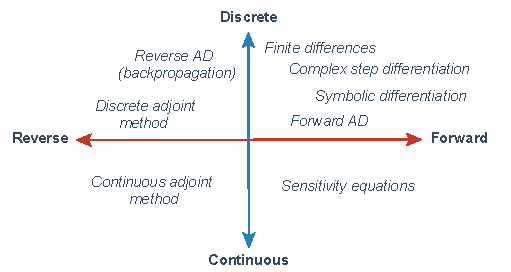
\includegraphics[width=0.80\textwidth]{figures/scheme-methods.pdf}
    \caption{Schematic representation of the different methods available for differentiation involving differential equation solutions. These can be classified depending if they find the gradient by solving a new system of differential equations (\textit{continuous}) or if instead they manipulate unit algebraic operations (\textit{discrete}). Furthermore, depending on if these methods run in the same direction as the numerical solver, we are going to be talking about \textit{backward} and \textit{forward} methods.}
    \label{fig:diff}
\end{figure}
Depending on the number of parameters and the complexity of the differential equation we are trying to solve, there are different methods to compute gradients with different numerical and computational advantages.
These methods can be roughly classified as:
\begin{itemize}
    \item \textit{Discrete} vs \textit{continuous} methods
    \item \textit{Forward} vs \textit{backward} methods
\end{itemize}
The first difference regards the fact that the method for computing the gradient can be either based on the manipulation of atomic operations that are easy to differentiate using the chain rule several times (discrete), in opposition to the approach of approximating the gradient as the numerical solution of a new set of differential equations (continuous).
Another way of conceptualizing this difference is by comparing them with the discretize-differentiate and differentiate-discretize approaches \cite{bradley2013pde, Onken_Ruthotto_2020, FATODE2014, Sirkes_Tziperman_1997}.   
We can either discretize the original system of ODEs in order to numerically solve it and then define the set of adjoint equations on top of the numerical scheme; or instead define the adjoint equation directly using the differential equation and then discretize both in order to solve \cite{Giles_Pierce_2000}.

The second distinction is related to the fact that some methods compute gradients by resolving a new sequential problem that may move in the same direction as the original numerical solver - i.e. moving forward in time - or, instead, they solve a new system that goes backwards in time. 
Figure \ref{fig:diff} displays a classification of some methods under this two-fold classification. In the following section, we are going to explore more in detail these methods.

It is important to note that if all the methods we explore in this section are mathematically correct, \textit{that does not imply they are numerically stable}.
These statements applied to methods based on pure automatic differentiation as well as adjoint methods. 
We are going to explore this consideration in more detail in section \ref{sec:computational-implementation}.

\subsection{Preliminaries}
Consider a system of ordinary differential equations (ODEs) given by
\begin{equation}
 \frac{du}{dt} = f(u, \theta, t),
 \label{eq:original_ODE}
\end{equation}
where $u \in \mathbb{R}^n$ is the unknown solution; $f$ is a function that depends on the state $u$, some parameter $\theta \in \mathbb R^p$, and an independent variable $t$ which we will refer as time, but it can represent another quantity; and with initial condition $u(t_0) = u_0$.
Here $n$ denotes the total number of ODEs and $p$ the size of a parameter embedded in the functional form of the differential equation.
Although here we consider the case of ODEs, that is, when the derivatives are just with respect to the time variable $t$, the ideas presented here can be extended of the case of partial differential equations (for example, via the method of lines \cite{ascher2008numerical}) and differential algebraic equations (DAE).
% Furthermore, the fact that both $u$ and $\theta$ are one-dimensional vectors does not prevent the use of higher-dimension objects (e.g. when $u$ is a matrix or a tensor). 
Except for a minority of functions $f(u,\theta, t)$, solutions of the Equation \eqref{eq:original_ODE} need to be computed using a numerical solver. 

We are interested in computing the gradient of a given function $L(u(\cdot, \theta))$ with respect to the parameter $\theta$.
Here we are using the letter $L$ to emphasize that in many cases this will be a loss function, but without loss of generality this includes a broader class of functions. 
% Maybe organize this in sections, like 
\begin{itemize}
    \item \textbf{Empirical loss functions}. This is usually a real-valued function that quantifies the level of agreement between the model prediction and the data. Examples of loss functions include the squared error
    \begin{equation}
         L(u(\cdot, \theta)) = \frac{1}{2} \| u(t_1; \theta) - u^{\text{target}}(t_1) \|_2^2,
         \label{eq:quadratic-loss-function}
    \end{equation}
    where $u^{\text{target}}(t_1)$ is the desired target observation at some later time $t_1$.
    More generally, we can evaluate the loss function at points of the time series for which we have observations, 
    \begin{equation}
        L(u(\cdot, \theta)) = \frac{1}{2} \sum_{i=1}^N \| u(t_i; \theta) - u^{\text{target}}(t_i) \|_2^2.
    \end{equation}
    We can also consider the continuous evaluated loss function of the form
    \begin{equation}
         L(u(\cdot, \theta)) = \int_{t_0}^{t_1} h( u(t;\theta), \theta) ) dt, 
    \end{equation}
    with $h$ being a function that quantifies the contribution of the error term at every time $t \in [t_0, t_1]$. 
    Defining a loss function where just the empirical error is penalized is known as trajectory matching. 
    Other methods like gradient matching and generalized smoothing the loss depends on smooth approximations of the trajectory and their derivatives. 
    \todo{this is unclear}
    \item \textbf{Likelihood profiles.} From a statistical perspective, it is common to assume that observations correspond to noisy observations of the underlying dynamical system, $y_i = u(t_i; \theta) + \varepsilon_i$, with $\varepsilon_i$ errors or residual that are independent of each other and of the trajectory $u(\cdot ; \theta)$ \cite{ramsay2017dynamic}.
    If $p(y | t , \theta)$ is the probability distribution of $y$, maximum likelihood estimation consists in finding the parameter $\theta$ as
    \begin{equation}
        \theta^* 
        = 
        \argmax{\theta} \, \ell (y | \theta) 
        = 
        \prod_{i=1}^n p(y_i | \theta, t_i) .
    \end{equation}
    When $\varepsilon \sim N(0, \sigma_i^2)$ is Gaussian, the maximum likelihood principle is the same as minimizing $- \log \ell(y | \theta)$ which results in the mean squared error
    \begin{equation}
        \theta^* 
        = 
        \argmin{\theta} \, \left \{ - \log \ell (y | \theta) \right \}
        = 
        \argmin{\theta} \, \sum_{i=1}^n \left( y_i - u(t_i; \theta) \right)^2 .
    \end{equation} % \todo[inline]{There is a correspondance between this equation and the empirical loss function above, which would be nice to show. See the proposed section "Maximum likelihood estimation and loss function". This is also discussed in e.g. https://www.deeplearningbook.org/contents/prob.html}
    Provided with a prior distribution $p(\theta)$ for the parameter $\theta$, we can further compute a posterior distribution for $\theta$ given the observations $y_1, y_2, \ldots, y_n$ following Bayes theorem 
    \begin{equation}
        p(\theta | y) = \frac{p(y | \theta) p (\theta)}{p(y)}. 
    \end{equation}
    In practice, the posterior is difficult to evaluate and needs to be approximated using Markov chain Monte Carlo sampling methods \cite{gelman2013bayesian}. being able to further compute gradients of the likelihood allows to design more efficient sampling methods, such as Hamiltonian MCMC \cite{Betancourt_2017}. 
    \item \textbf{Quantity of interest.} Another important example is when $L$ returns the value of the solution at one or many points, which is useful when we want to know how the solution itself changes as we move the parameter values. 
    \item \textbf{Diagnosis of the solution.} In many cases we are interested in optimizing the value of some variable that is a function of the solution of a differential equation. This is the case in design control theory, a popular approach in aerodynamics modelling where goals include maximizing the speed of an airplane or the lift of a wing given the solution of the flow equation for a given geometry profile \cite{Jameson_1988}. 
\end{itemize}

In this context, the gradient of the loss allows performing gradient-based updates on the parameter $\theta$ by 
\begin{equation}
    \theta^{k+1} 
    = 
    \theta^k 
    - 
    \alpha_k 
    \frac{dL}{d\theta^k}.
\end{equation}
Gradient-based methods tend to outperform gradient-free optimization schemes, as they are not prone to the curse of dimensionality \cite{Schartau2017}. 
While a direct implementation of gradient descent is prone to converge to a local minimum and slow down in a neighborhood of saddle points, variants employing more advanced updating strategies have been proposed \cite{ruder2016overview-gradient-descent} to avoid convergence to local minima, and are widely adopted in the field of artificial intelligence to train highly parametrized neural networks (up to the order of $10^8$ parameters \cite{NIPS2017_3f5ee243}). 
For instance, Adam \cite{Kingma2014} is an adaptive, momentum-based algorithm  that remembers the solution update at each iteration, and determines the next update as a linear combination of the gradient and the previous update, reducing the risk to converge to local minima. 
Other broadly employed algorithms are the Broyden–Fletcher–Goldfarb–Shanno (BFGS) and its limited-memory version algorithm (L-BFGS), which determine the descent direction by preconditioning the gradient with curvature information. 
ADAM is less prone to converging to a local minimum, while (L-)BFGS has a faster converge rate. 
Using ADAM for the first iterations followed by (L-)BFGS proves to be a successful strategy to minimize a loss function with best accuracy. 
% Furthermore, gradient-free methods (also known as global optimization techniques \todo{Some gradient free methods are not necessarily global optimization techniques, e.g. evolutionary algorithms \cite{wilke2001evolution,Rodriguez-Fernandez2006} }) rely in heuristics\cite{Pearl-heuristics} that are not guaranteed to find the solution. 

% \subsubsection{Sensitivity matrix}
Using the chain rule we can derive
\begin{equation} 
 \frac{dL}{d\theta} = \frac{dL}{du} \frac{\partial u}{\partial \theta}.
 \label{eq:dLdtheta_VJP}
\end{equation} 
The first term on the right-hand side is usually easy to evaluate since it just involves the partial derivative of the scalar loss function with respect to the solution.
For example, for the loss function in Equation \eqref{eq:quadratic-loss-function} this is simply
\begin{equation}
    \frac{dL}{du} = u - u^{\text{target}}(t_1).
    \label{eq:dLdu}
\end{equation}
The second term on the right-hand side is more difficult to compute and it is usually referred to as the \textit{sensitivity},
\begin{equation}
 s 
 = 
 \frac{\partial u}{\partial \theta} 
 =
 \begin{bmatrix}
   \frac{\partial u_1}{\partial \theta_1} & \dots & \frac{\partial u_1}{\partial \theta_p} \\
   \vdots & \ddots & \vdots \\
   \frac{\partial u_n}{\partial \theta_1} & \dots & \frac{\partial u_n}{\partial \theta_p}
 \end{bmatrix}
 \in \mathbb R^{n \times p}.
 \label{eq:sensitivity-definition}
\end{equation}
Notice here the distinction between the total derivative (indicated with the $d$) and partial derivative symbols ($\partial$). 
When a function depends on more than one argument, we use the partial derivative symbol to emphasize this distinction (e.g., Equation \eqref{eq:sensitivity-definition}). 
On the other side, when this is not the case, we will use the total derivative symbol (e.g., Equation \eqref{eq:dLdu}).
Also notice that the sensitivity $s$ defined in Equation \eqref{eq:sensitivity-definition} is what is called a \textit{Jacobian}, that is, a matrix of first derivatives for general vector-valued functions.

% In this article we are going to use the word gradient or derivative to refer to the first order derivatives of a given function. 
% Although the names adjoint and tangent are sometime used to refer to the same object, we are going to skip the use of these to avoid confusion.
% The same nature of the adjoint methods deserves to be treated entirely in Section \ref{section:adjoint-methods}.


\subsection{Finite differences}
The simplest way of evaluating a derivative is by computing the difference between the evaluation of the function at a given point and a small perturbation of the function. 
In the case of the function $L : \R^p \mapsto \R$, we can approximate
\begin{equation}
 \frac{dL}{d\theta_i} (\theta) = \frac{L(\theta + \varepsilon e_i ) - L(\theta)}{\varepsilon} + \mathcal O (\varepsilon),
 \label{eq:finite_diff}
\end{equation}
with $e_i$ the $i$-th canonical vector and $\varepsilon$ the stepsize. 
Even better, the centered difference scheme leads to
\begin{equation}
 \frac{dL}{d\theta_i} (\theta) 
 =
 \frac{L(\theta + \varepsilon e_i ) - L(\theta - \varepsilon e_i)}{2\varepsilon}
 + \mathcal O (\varepsilon^2).
 \label{eq:finite_diff2}
\end{equation}
% leads to a more accurate estimation of the derivative. 
While Equation \eqref{eq:finite_diff} gives the derivative to an error of magnitude $\mathcal O (\varepsilon)$, the centered differences schemes improves the accuracy to $\mathcal O (\varepsilon^2)$ \cite{ascher2008-numerical-methods}. 
Further finite difference stencils of higher order exist in the literature \cite{Fornberg1988}. 
 
However, there are a series of problems associated with finite differences when seeking to compute the gradient of $L$.
The first is due to how it scales with the dimension $p$ of parameter vector $\theta$.
Each directional derivative requires at least one extra evaluation of the loss function.
For the centered differences approach in Equation \eqref{eq:finite_diff2}, this requires a total of $2p$ function evaluations which demands solving the differential equation each time for a new set of parameters.
A second problem is rounding errors.
Every computer ultimately stores and manipulates numbers using floating point arithmetic \cite{Goldberg_1991_floatingpoint}. 
Equations \eqref{eq:finite_diff} and \eqref{eq:finite_diff2} involve the subtraction of two numbers that are very close to each other, which leads to large cancellation errors for small values of $\varepsilon$ that are amplified by the division by $\varepsilon$.
On the other hand, large values of the stepsize give inaccurate estimations of the gradient. 
Finding the optimal value of $\varepsilon$ that balances these two effects is sometimes known as the \textit{stepsize dilemma}, for which algorithms based on prior knowledge of the function to be differentiated or algorithms based on heuristic rules have been introduced \cite{mathur2012stepsize-finitediff, BARTON_1992_finite_diff, SUNDIALS-hindmarsh2005sundials}. 
% \todo{Would be nice to show more formally the effect of the round-off error, see e.g. https://book.sciml.ai/notes/08-Forward-Mode_Automatic_Differentiation_(AD)_via_High_Dimensional_Algebras/}
% Some of these methods require some prior knowledge of the function to be differentiated, and others are based on heuristic rules. 
If well many analytical functions, like polynomials and trigonometric functions, can be computed with machine precision, numerical solutions of differential equations have errors that are typically larger than machine precision, which leads to inaccurate estimations of the gradient when $\varepsilon$ is too small. 
We will further emphasize this point in Section \ref{sec:computational-implementation}.

Despite all these caveats, finite differences can be useful when computing Jacobian-vector products (JVPs). 
Given a Jacobian matrix $J = \frac{\partial f}{\partial u}$ (or the sensitivity $s = \frac{\partial u}{\partial \theta}$) and a vector $v$, the product $Jv$ corresponding to the directional derivative and can be approximated as 
\begin{equation}
    Jv \approx \frac{f(u + \varepsilon v, \theta, t) - f(u, \theta, t)}{\varepsilon}
\end{equation}
This approach is used in numerical solvers based on Krylov methods, where linear systems are solved by iteratively solving matrix-vectors products \cite{Ipsen_Meyer_1998}.

% Replacing derivatives by finite differences is also a common practice when solving partial differential equations (PDEs), a technique known as the \textit{method of lines} \cite{ascher2008numerical}. 
% To illustrate this point, let us consider the case of the one-dimensional heat equation
% \begin{equation}
%  \frac{\partial u}{\partial t}
%  = 
%  D \, 
%  \frac{\partial^2 u}{\partial x^2}, 
%  \quad u(0, t) = \alpha(t), 
%  \quad u(1, t) = \beta(t)
%  \label{eq:heat-equation}
% \end{equation}
% that includes both spatial and temporal partial derivatives of the unknown function $u(x, t)$.
% In order to numerically solve this equation, we can define a spatial grid with coordinates $m \Delta x$, $m=0, 1, 2, \ldots, N$ and $\Delta x = 1 / N$.
% If we call $u_m(t) = u(m \Delta x, t)$ the value of the solution evaluated in the fixed points in the grid, then we can replace the second order partial derivative in Equation \eqref{eq:heat-equation} by the corresponding second order finite difference\footnote{Since $u_m(t)$ is a function of one single variable, we write the total derivative $\frac{du_m}{dt}$ instead of the partial derivative symbol used before $\frac{\partial u}{\partial t}$, which it is usually used just for multivariable function.}
% \begin{equation}
%  \frac{d u_m}{dt} 
%  = 
%  D 
%  \frac{u_{m-1} - 2u_m + u_{m+1}}{\Delta x^2}
%  \label{eq:heat-equation-discrete}
% \end{equation}
% for $m = 1, 2, \ldots, N-1$ (in the extremes we simply have $u_0(t) = \alpha(t)$ and $u_N(t)=\beta(t)$).
% Now, equation \eqref{eq:heat-equation-discrete} is a system of ordinary differential equations (just temporal derivatives) with a total of $N-1$ equations.
% This can be solved directly using an ODE solver.
% Further improvements can be made by exploiting the fact that the coupling between the different functions $u_m$ is sparse, that is, the temporal derivative of $u_m$ just depends of the values of the function in the neighbour points in the grid.



\subsection{Complex step differentiation}
An alternative to finite differences that avoids rounding errors is based complex variable analysis. 
The first proposals originated in 1967 using the Cauchy integral theorem involving the numerical evaluation of a complex valued integral \cite{Lyness_1967, Lyness_Moler_1967} .
A new approach recently emerged that uses the Taylor expansion of a function to define its complex generalization \cite{Squire_Trapp_1998_complex_diff}. 
Assuming that we have one single scalar parameter $\theta \in \R$, then the function $L(\theta)$ can be expanded as 
the Taylor expansion
\begin{equation}
    L(\theta + i \, \varepsilon)
    = 
    L(\theta) + i \varepsilon L'(\theta) 
    - 
    \frac 1 2
    L''(\theta) \varepsilon^2
    + 
    \mathcal O (\varepsilon^3),
\end{equation}
where $i$ is the imaginary unit with the property $i^2 = -1$. 
From this equation we can observed that many factors vanish when we compute the imaginary part $\text{Im}(L(\theta + i \varepsilon))$, which leads to
\begin{equation}
    L'(\theta) 
    = 
    \frac{\text{Im}(L(\theta + i \varepsilon))}{\varepsilon}
    + 
    \mathcal{O} (\varepsilon^2)
\end{equation}
The method of \textit{complex step differentiation} consist then in estimating the gradient as $\text{Im}(L(\theta + i \varepsilon)) / \varepsilon$ for a small value of $\varepsilon$. 
Besides the advantage of being a method with precision $\mathcal{O}(\varepsilon^2)$, the complex step method avoids subtracting cancellation error and then the value of $\varepsilon$ can be reduce to almost machine precision error without affecting the calculation of the derivative. 

Extension to higher order derivatives can be done by introducing multicomplex variables \cite{Lantoine_Russell_Dargent_2012}. 

Other authors had suggested to use complex variable analysis to compute the derivative as the imaginary part of $L(\theta + i \varepsilon)/h$, which coincides with $L'(\theta)$ for the case where $\theta$ is a scalar \cite{ Martins_Sturdza_Alonso_2003_complex_differentiation}.
% This approach was later generalized to the multivariable case 
Although this solves the problem of cancellation errors in Equation \eqref{eq:finite_diff2} for small $\varepsilon$, this approach is just valid for cases where the function $L$ is known analytically. 


\subsection{Automatic differentiation}
% I think I need some historical reference here.
Automatic differentiation (AD) is a technology that allows computing gradients thought a computer program \cite{griewank2008evaluatingderivatives}. 
The basis of all AD system is the notion that complicated functions included in any computer program can be reduced to a sequence of simple algebraic operations that have straightforward derivative expressions, based upon elementary rules of differentiation \cite{juedes1991taxonomy}.
The derivatives of the outputs of the computer program with respect to their inputs are then combined using the chain rule.
One advantage of AD systems is that we can automatically differentiate programs that include control flow, such as branching, loops or recursions. 
This is because at the end of the day, any program can be reduced to a trace of input, intermediate and output variables \cite{Baydin_Pearlmutter_Radul_Siskind_2015}.

Depending if the concatenation of these gradients is done as we execute the program (from input to output) or in a later instance were we trace-back the calculation from the end (from output to input), we are going to talk about \textit{forward} or \textit{reverse} AD, respectively.
Neither forward or reverse mode is more efficient in all cases \cite{Griewank_1989}, as we will discuss in Section \ref{sec:vjp-jvp}.

\subsubsection{Forward mode}

Forward mode AD can be implemented in different ways depending on the data structures we use at the moment of representing a computer program. Examples of these data structures include dual numbers and Wengert lists (see \cite{Baydin_Pearlmutter_Radul_Siskind_2015} for a good review on these methods). 

\vspace*{10px}
\noindent \textbf{\textit{Dual numbers}}
\vspace*{5px}

Dual numbers extend the definition of a numerical variable that takes a certain value to also carry information about its derivative with respect to certain parameter \cite{clifford1871dualnumbers}. 
We can define an abstract type, defined as a dual number, composed of two elements: a \textit{value} coordinate $x_1$ that carries the value of the variable and a \textit{derivative} coordinate $x_2$ with the value of the derivative $\frac{\partial x_1}{\partial \theta}$. 
Just as complex number, we can represent dual numbers as an ordered pair $(x_1, x_2)$, sometimes known as Argand pair, or in the rectangular form 
\begin{equation}
 x_\epsilon = x_1 + \epsilon \, x_2
\end{equation}
where $\epsilon$ is an abstract number called a perturbation or tangent, with the properties $\epsilon^2 = 0$ and $\epsilon \neq 0$.
This last representation is quite convenient since it naturally allow us to extend algebraic operations, like addition and multiplication, to dual numbers \cite{Karczmarczuk2001}. 
For example, given two dual numbers $x_\epsilon = x_1 + \epsilon x_2$ and $y_\epsilon = y_1 + \epsilon y_2$, it is easy to derive using the fact $\epsilon^2=0$ that
\begin{equation}
 x_\epsilon + y_\epsilon = (x_1 + y_1) + \epsilon \, (x_2 + y_2)
 \qquad
 x_\epsilon y_\epsilon = x_1 y_1 + \epsilon \, (x_1 y_2 + x_2 y_1) .
 %\qquad
 %\frac{x_\epsilon}{y_\epsilon} = \frac{x_1}{y_1} + \epsilon \, \frac{x_2 y_1 - x_1 y_2}{y_1^2}.
\end{equation}
From these last examples, we can see that the derivative component of the dual number carries the information of the derivatives when combining operations.
For example, suppose than in the last example the dual variables $x_2$ and $y_2$ carry the value of the derivative of $x_1$ and $x_2$ with respect to a parameter $\theta$, respectively. 

Intuitively, we can think about $\epsilon$ as being a differential in the Taylor expansion:
\begin{align}
    f(x_1 + \epsilon x_2)
    &= 
    f(x_1)
    + 
    \epsilon \, x_2 \,  f'(x_1)
    + 
    \epsilon^2 \cdot ( \ldots ) \nonumber \\
    &= 
    f(x_1)
    + 
    \epsilon \, x_2 \,  f'(x_1)
    \label{eq:dual-number-function}
\end{align}
When computing first order derivatives, we can ignore everything of order $\epsilon^2$ or larger, which is represented in the condition $\epsilon^2 = 0$.
This implies that we can use dual numbers to implement forward AD through a numerical algorithm. 
In Section \ref{sec:computational-implementation} we will explore how this is implemented and compare this approach with complex-step differentiation. 

\vspace*{10px}
\noindent \textbf{\textit{Computational graph}}
\vspace*{5px}

A useful way of representing a computer program is via a computational graph with intermediate variables that relate the input and output variables. 
Most scalar functions of interest can be represented in this factorial form as a acyclic directed graph with nodes associated to variables and edges to atomic operations \cite{griewank2008evaluatingderivatives, Griewack-on-AD}, known as Kantorovich graph \cite{kantorovich1957mathematical} or Wengert trace/tape\cite{Wengert_1964, Bauer_1974}. 
% Although notation can be a little bit difficult to digest here, the mathematics behind is rather simple. 
We can define $v_1, v_2, \ldots, v_p = \theta_1, \theta_2, \ldots, \theta_p$ the input set of variables; $v_{p+1}, \ldots, v_{m-1}$ the set of all the intermediate variables, and finally $v_m = L(\theta)$ the final output of a computer program. 
This can be done in such a way that the order is strict, meaning that each variable $v_i$ is computed just as a function of the previous variables $v_j$ with $j < i$. 
Once the graph is constructed, we can compute the derivative of every node with respect to other (a quantity known as the tangent) using Bauer formula \cite{Bauer_1974, Oktay_randomized-AD}
\begin{equation}
    \frac{\partial v_j}{\partial v_i}
    = 
    \sum_{\substack{ \text{paths }w_0 \rightarrow w_1 \rightarrow \ldots \rightarrow w_K \\
                    \text{with } w_0=v_i, w_K = v_j}}
    \prod_{k=0}^{K-1} \frac{\partial w_{k+1}}{\partial w_{k}},
\end{equation}
where the sum is calculated with respect to all the directed paths in the graph connecting the input and target node.
Instead of evaluating the last expression for all possible path, a simplification is to increasingly evaluate $j=p+1, \ldots, m$ using the recursion 
\begin{equation}
    \frac{\partial v_j}{\partial v_i}
    = 
    \sum_\text{$w$\text{ such that} $w \rightarrow v_j$}
    \frac{\partial v_j}{\partial w}
    \frac{\partial w}{\partial v_i} 
    \label{eq:AD-graph-recursion}
\end{equation}
Since every variable node $w$ such that $w \rightarrow v_j$ is an edge of the computational graph have index less than $j$, we can iterate this procedure as we run the computer program and solve for both the function and its gradient.
This is possible because in forward mode the term $\frac{\partial w}{\partial v_i}$ has been computed in a previous iteration, while $\frac{\partial v_j}{\partial w}$ can be evaluated at the same time the node $v_j$ is computed based on only the value of the parent variable nodes. 
The only requirement for differentiation is being able to compute the derivative/tangent of each edge/primitive and combine these using the recursion \eqref{eq:AD-graph-recursion}.

\subsubsection{Backward mode}

Backward mode AD is also known as the adjoint of cotangent linear mode or backpropagation in the field of machine learning. 
The reverse mode of automatic differentiation has been introduced in different contexts \cite{griewank2012invented} and materializes the observation made by Phil Wolfe that if the chain rule is implemented in reverse mode, then the ratio between the computation of the gradient of a function and the function itself can be bounded by a constant that do not depend of the number of parameters to differentiate \cite{Griewack-on-AD, Wolfe_1982}, a point known as \textit{cheap gradient principle} \cite{griewank2012invented}.  
Given a directional graph of operations defined by a Wengert list \cite{Wengert_1964}, we can compute gradients of any given function in the same fashion as Equation \eqref{eq:AD-graph-recursion} but in backwards mode as
\begin{equation}
 \bar v_i = \frac{\partial \ell}{\partial v_i}= \sum_{w : v \rightarrow w \in G} \frac{\partial w}{\partial v} \bar{w}.
\end{equation}
Here we have introduced the notation $\bar{\omega} = \frac{\partial \ell}{\partial \omega}$ to indicate that the partial derivative is always of the final loss function with respect to the different program variables, a quantity sometimes refers as adjoint (do not confuse with the adjoint method of later sections) or cotangent. 
Since in backwards AD the values of $\bar \omega$ are being updated in reverse order, in order to evaluate the terms $\frac{\partial \omega}{\partial v}$ we need to know the state value of all the argument variables $v$ of $\omega$, which need to be stored in memory during the evaluation of the function in order to be able to apply backward AD.


\subsubsection{AD connection with JVPs and VJPs}
\label{sec:vjp-jvp}

When working with unit operations that involve matrix operations dealing with vectors of different dimensions, the order in which we apply the chain rule matters \cite{Giering_Kaminski_1998}.
When computing a gradient using AD, we can encounter vector-Jacobian products (VJPs) or Jacobian-vector products (JVP).
As their name indicates, the difference between them regards the fact that the quantity we are interested in computing is described by the product of a Jacobian by a vector on the left side (VJP) or the right (JVP).

For nested functions, the Jacobian is described as the product of multiple Jacobians using the chain rule.
In this case, the full gradient is computed as the chain product of vectors and Jacobians. 
Let us consider for example the case of a loss function $L : \mathbb R^p \mapsto \mathbb R$ taking a total of $p$ arguments as inputs that can be decomposed as $L(\theta) = \ell \circ g_{k} \circ \ldots \circ g_2 \circ g_1(\theta)$, with $\ell : \mathbb R^{d_k} \mapsto \mathbb R$ the final evaluation of the loss function after we apply in order a sequence of intermediate functions $g_i : \mathbb R^{d_{i-1}} \mapsto \mathbb R^{d_i}$, where we define $d_0 = p$ for simplicity. 
Using the chain rule states that the gradient of the final loss function is
\begin{equation}
 \nabla_\theta L = \nabla \ell \cdot Dg_{k} \cdot Dg_{k-1} \cdot \ldots \cdot Dg_2 \cdot Dg_1, 
\end{equation}
with $Dg_i$ the Jacobians of each nested function. 
Notice that in the last equation, $\nabla \ell \in \mathbb R^{d_k}$ is a vector.
In order to compute $\nabla_\theta L$, we can solve the multiplication starting from the right side, which will correspond to multiplying the Jacobians forward from $Dg_1$ to $Dg_k$, or from the left side, moving backwards. 
The important aspect of the backwards case is that we will always be computing VJPs, since $\nabla \ell$ is a vector.
Since VJPs are easier to evaluate than full Jacobians, the backward mode will be in general faster when $1 \ll p$.
To illustrate this, let us consider the following example displayed in Figure \ref{fig:vjp-jvp}. 
For general rectangular matrices $A\in \mathbb R^{d_1 \times d_2}$ and $B \in \mathbb R^{d_2 \times d_3}$, the cost of the matrix multiplication $AB$ is $\mathcal O (d_1 d_2 d_3)$.
It is worth noticing that if well more efficient methods for matrix-matrix multiplication based on Strassen’s recursive algorithm and its variants exist, these are not extensively used in most scientific applications \cite{Silva_Gustafson_Wong_2018, Huang_Smith_Henry_Geijn_2016}.
This implies that forward AD requires a total of
\begin{equation}
 d_2 d_1 p + d_3 d_2 p + \ldots + d_k d_{k-1} p + d_k p = \mathcal O (kp)
\end{equation}
operations, while backwards mode AD requires
\begin{equation}
 d_k d_{k-1} + d_{k-1} d_{k-2} + \ldots + d_2 d_1 + d_1 p = \mathcal O (k+p)
\end{equation}
operations, where the $\mathcal O$ is with respect to the variable $p$. 

In the general case of a function $L : \R^p \mapsto \R^q$ with multiple outputs and a total of $k$ intermediate functions, the cost of forward AD is $\mathcal O (pk + q)$ and the cost of reverse is $\mathcal O (p + kq)$.
When the function to differentiate has a larger input space than output ($q \ll p$), AD in backward mode is more efficient as it propagates the chain rule by computing VJPs, the reason why backwards AD is more used in modern machine learning.
% On the other side, when the output dimension is larger than the input space dimension, forwards AD is more efficient.
% This is the reason why in most machine learning application people use backwards AD. 
However, notice that backwards mode AD requires us to save intermediate variables through the forward run in order to run backwards afterwards \cite{Bennett_1973}, leading to performance overhead that makes forward AD more efficient when $p \lesssim q$ \cite{Griewank_1989, Margossian_2018, Baydin_Pearlmutter_Radul_Siskind_2015}.  
In other words, backwards AD is really more efficient when $q \ll p$. 
% while in forward mode we can just evaluate the gradient as we iterate our sequence of functions. 
This problem can be mitigated, to some extent, with a good checkpointing scheme we will discuss later. 
% On the other hand, when the goal is to compute the gradient of many function outputs with respect to a few parameters, forward mode AD is more efficient \cite{Griewank_1989}.
% This means that for problems with a small number of parameters, forward mode can be faster and more memory-efficient that backwards AD.

\begin{figure}[t]
    \centering
    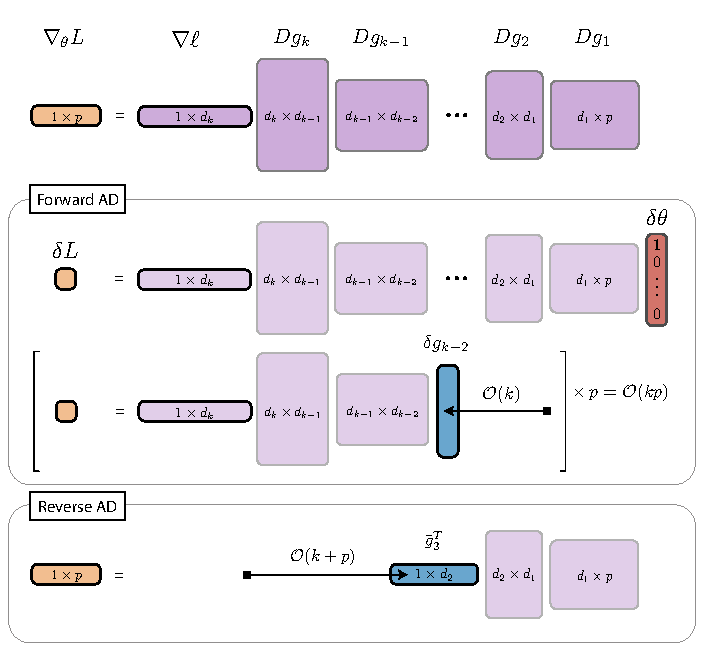
\includegraphics[width=0.95\textwidth]{tex/figures/VJP-AD.pdf}
    \caption{Comparison between forward and backward AD. Changing the order of how we multiply the Jacobians change the total number of floating-point operations, which leads to different computational complexities between forward and backward mode. When the multiplication is carried from the right side of the mathematical expression for $\nabla_\theta L$, each matrix simplification involves a matrix with size $p$, giving a total complexity of $\mathcal O (kp)$. This is the opposite of what happens when we carried the VJP from the left side of the expression, where the matrix of size $d_1 \times p$ has not affect in the intermediate calculations, making all the intermediate calculations $\mathcal O (1)$ with respect to $p$ and a total complexity of $\mathcal O (k + p)$. }
    % However, backwards mode requires storing in memory information about the forward execution of the program, while forward mode can update the gradient on running time.}
    \label{fig:vjp-jvp}
\end{figure}


\subsection{Symbolic differentiation}
In symbolic differentiation, functions are represented algebraically instead of algorithmically, reason why many symbolic differentiation tools are included inside computer algebra systems (CAS)\cite{Symbolics_jl_2022}. 
Instead of numerically evaluating the final value of a derivative, symbolic systems define \textit{algebraic} objects, including variable names, expressions, operations, and literals. 
For example, the relation $y = x^2$ is interpreted as expression with two variables, $x$ and $y$, and the symbolic system need to generate the derivative $y' = 2 \times x$ with $2$ a numeric literal, $\times$ a binary operation, and $x$ the same variable assignment than in the original expression.
When the function to differentiate is large, symbolic differentiation can lead to \textit{expression swell}, that is, exponentially large or complex symbolic expressions \cite{Baydin_Pearlmutter_Radul_Siskind_2015}.
Here, an important piece of CAS is simplification routines that reduce the size and complexity of algebraic expressions by finding common sub-expressions.  
This can make symbolic differentiation very efficient when computing derivatives multiple times and for different input values \cite{Dürrbaum_Klier_Hahn_2002}. 

It is important to remark the close relationship between AD and symbolic differentiation.
There is not agreement weather symbolic differentiation should be classified as AD\cite{juedes1991taxonomy, Elliott_2018, Laue2020} or as a different method \cite{Baydin_Pearlmutter_Radul_Siskind_2015}.  
Both are equivalent in the sense that they perform the same operations but the underlying data structure is different \cite{Laue2020}. 
Here, expression swell is a consequence of the underlying representation when this does not allow for common sub-expressions. 
This can also been understood as if AD is symbolic differentiation performed by a compiler \cite{Elliott_2018}, meaning that different AD can be classified based in the level of integration with the underlying source language \cite{juedes1991taxonomy}.
% This means that the mathematical calculations involved are the same, but they need to be interpreted by the compiler at the moment of computing the derivative. 
% Something like $x + 2$ needs to be understood as an \textit{expression} composed by a variable $x$, a literal $2$, and a binary operation $+$ binding them. 



\subsection{Sensitivity equations}
An easy way to derive an expression for the sensitivity $s$ defined in Equation \eqref{eq:sensitivity-definition} is by deriving the forward sensitivity equations \cite{ramsay2017dynamic}, a method also referred to as continuous local sensitivity analysis (CSA). 
If we consider the original ODE given by Equation \eqref{eq:original_ODE} and we differentiate with respect to $\theta$, we then obtain
\begin{equation}
    \frac{d}{d\theta} \left( \frac{du}{dt}  - f(u(\theta), \theta, t) \right) = 0.
\end{equation}
Assuming that a unique solution exists and both $\frac{\partial f}{\partial u}$ and $\frac{\partial f}{\partial \theta}$ are continuous in the neighbourhood of the solution, or under the guarantee of interchangeability of the derivatives \cite{gronwall1919note}, for example by assuming that both $\frac{du}{dt}$ and $\frac{du}{d\theta}$ are differentiable \cite{math8111947}, we can derive
\begin{equation}
 \frac{d}{d\theta} \frac{du}{dt} 
 =
 \frac{d}{d\theta} f(u(\theta), \theta, t)
 = 
 \frac{\partial f}{\partial \theta}
 + 
 \frac{\partial f}{\partial u} \frac{\partial u}{\partial \theta}.
\end{equation}
Identifying the sensitivity matrix $s(t)$ now as a function of time, we obtain the \textit{sensitivity differential equation} 
\begin{equation}
 \frac{ds}{dt} = \frac{\partial f}{\partial u} s + \frac{\partial f}{\partial \theta}.
 \label{eq:sensitivity_equations}
\end{equation}
The initial condition is simply given by $s(t_0) = \frac{du_0}{d\theta}$, which is zero unless the initial condition explicitly depends on the parameter $\theta$.
Both the original ODE of size $n$ and the forward sensitivity equation with size $np$ are solved simultaneously, which is necessary since the forward sensitivity DE directly depends on the value of $u(t)$.  
This implies that as we solve the ODE, we can ensure the same level of numerical precision for the two of them inside the numerical solver.

In contrast to the methods previously introduced, the forward sensitivity equations find the derivative by solving a new set of continuous differential equations.
Notice also that the obtained sensitivity $s(t)$ can be evaluated at any given time $t$. 
This method can be labeled as forward, since we solve both $u(t)$ and $s(t)$ as we solve the DE forward in time, without the need of backtracking any operation though the solver.
By solving the forward sensitivity equation and the original ODE for $u(t)$ simultaneously, we ensure that by the end of the forward step we have calculated both $u(t)$ and $s(t)$. 

\subsection{Adjoint methods}
\label{section:adjoint-methods}
For complex and large systems, computing the gradient directly on top of the numerical solver (for example, using AD) can be memory expensive since the large number of function evaluation required by the solver and the later store of the intermediate states. 
For these cases, adjoint-based method allow to compute the gradients of a loss function by instead computing an intermediate variable (the adjoint) that serves as a bridge between the solution of the ODE and the final sensitivity. 
There is a large family of adjoint methods that a first order we can classify them between discrete and continuous adjoints. 
The former usually arises as the numerical discretization of the later, and when the discrete adjoint method is a consistent estimator of the continuous adjoint depends of the ODE and equation.  
Proofs of the consistency of discrete adjoint methods for Runge-Kutta methods had been provided in \cite{sandu2006properties, sandu2011solution}.
Depending the choice of the Runge-Kutta coefficients, we can have a numerical scheme that is both consistent for the original equation and consistent/inconsistent for the adjoint \cite{Hager_2000}.

\subsubsection{Discrete adjoint method}
Also know as the adjoint state method, it is another example of a discrete method that aims to find the gradient by solving an alternative system of linear equations, known as the \textit{adjoint equations}, at the same time that we solve the original system of linear equations defined by the numerical solver. 
These methods are extremely popular in optimal control theory in fluid dynamics, for example for the design of geometries for vehicles and airplanes that optimize performance \cite{Elliott_Peraire_1996, Giles_Pierce_2000}.
This approach follows the discretize-optimize approach, meaning that we first discretize the system of continuous ODEs and then solve on top of these linear equations \cite{Giles_Pierce_2000}. 

% Just as in the case of automatic differentiation, the adjoint state method evaluates the gradient by moving forward in time and applying the chain rule sequentially over a discrete set of operations that dictate the updates by the numerical scheme for solving the differential equation. However, it does so by directly computing the gradient by solving a new system of equations.

% Mathematically, reverse mode AD is related to the adjoint differential equations \cite{Griewack-on-AD}

\vspace*{10px}
\noindent \textbf{\textit{Discrete differential equation}}
\vspace*{5px}

% reference: Sensitivity theory of non-linear systems

The first step in order to derive the adjoint equation is to discretize the ODE in Equation \eqref{eq:original_ODE} into finite evaluations of the function $u(t; \theta)$. 
Given the sequence of timesteps $t_0, t_1, \ldots, t_N$, we evaluate the solution at $u_i = u(t_i; \theta)$. 
Most commonly used numerical solver consists in linear multisteps methods with the form 
\begin{equation}
    \sum_{i=1}^{K_1} \alpha_{n,i} u_{n-i} 
    +
    h_n \sum_{i=1}^{K_2} \beta_{n,i} f(u_{n-i}, \theta, t_i)
    = 
    0
\end{equation}
In the case of using an explicit numerical solver, these values will be constrained to satisfy a set of equations of the form 
\begin{equation}
    u_{i+1} = A_i (\theta) \, u_i + b_i
\end{equation}
with $A_i \in \R^{n \times n}$ a squared matrix defined by the numerical solver. 
Solving the differential equation then implies to be able to solve the system of constraints 
\begin{equation}
    g_i (u_{i+1}; \theta) = u_{i+1} - A_i (\theta) \, u_i - b_i = 0
\end{equation}
for all $i=0, 1, \ldots, N-1$. 
For most cases, this system can be solved sequentially, by solving for $u_i$ in increasing order of index. 
If we call the super-vector $U = (u_1, u_2, \ldots, u_N) \in \R^{nN}$, we can combine all these equations in into one single system of linear equations 
\begin{equation}
    A(\theta) U 
    = 
    \begin{bmatrix}
        \I_{n \times n} & 0 &   &  & \\
        -A_1 & \I_{n \times n} & 0 &  &  \\
          & -A_2 & \I_{n \times n} & 0 &  \\
         &  &   & \ddots &   \\
         &  &  & -A_{N-1} & \I_{n \times n}
    \end{bmatrix}
    \begin{bmatrix}
        u_1 \\
        u_2 \\
        u_3 \\
        \vdots \\
        u_N
    \end{bmatrix}
    = 
    \begin{bmatrix}
        A_0 u_0 + b_0 \\
        b_1 \\
        b_2 \\
        \vdots \\
        b_{N-1}
    \end{bmatrix}
    = 
    b(\theta), 
\end{equation}
with $\I_{n \times n}$ the identity matrix of size $n \times n$.
It is usually convenient to write this system of linear equations in the residual form $G(U; \theta) = 0$, where $G(U; \theta) = A(\theta) U - b(\theta)$ is the residual between both sides of the equation. 
Different numerical schemes will lead to different design matrix $A(\theta)$ and vector $b(\theta)$, but ultimately every numerical method will lead to a system of linear equations with the form $G(U; \theta) = A(\theta) U - b(\theta) = 0$ after being discretized. 
It is important to notice that in most cases, the matrix $A(\theta)$ is quite large and mostly sparse. 
If well this representation of the discrete differential equation is quite convenient for mathematical manipulations, at the moment of solving the system we will rely in iterative solvers that save memory and computation. 

\vspace*{10px}
\noindent \textbf{\textit{Adjoint state equations}}
\vspace*{5px}

We are interested in differentiating a function $L(U, \theta)$ with respect to the parameter $\theta$. 
Since here $U$ is the discrete set of evaluations of the solution, examples of loss functions now include 
\begin{equation}
    L(U, \theta) 
    = 
    \frac{1}{2} \sum_{i=1}^N \| u_i - u_i^\text{obs} \|^2, 
\end{equation}
with $u_i^\text{obs}$ the observed time-series. 
We further need to impose the constraint that the solution satisfies the algebraic linear equation $G(U; \theta) = 0$.
Now,
\begin{equation}
    \frac{dL}{d\theta} 
    = 
    \frac{\partial L}{\partial \theta} 
    + 
    \frac{\partial L}{\partial U} \frac{\partial U}{\partial \theta},
    \label{eq:dhdtheta0}
\end{equation}
and also for the constraint $G(U; \theta)=0$ we can derive
\begin{equation}
    \frac{dG}{d\theta} 
    = 
    \frac{\partial G}{\partial \theta} 
    + 
    \frac{\partial G}{\partial U} \frac{\partial U}{\partial \theta}
    =
    0
\end{equation}
which is equivalent to 
\begin{equation}
    \frac{\partial U}{\partial \theta} 
    = 
    - \left( \frac{\partial G}{\partial U} \right)^{-1} \frac{\partial G}{\partial \theta}.
\end{equation}
If we replace this last expression into equation \eqref{eq:dhdtheta0}, we obtain
\begin{equation}
    \frac{dL}{d\theta} 
    =
    \frac{\partial L}{\partial \theta} 
    - 
    \underbrace{\frac{\partial L}{\partial U}}_{\text{vector}}
    \left( \frac{\partial G}{\partial U} \right)^{-1} 
    \frac{\partial G}{\partial \theta}.
    \label{eq:dhdtheta}
\end{equation}
The important trick in the adjoint state methods is to observe that in this last equation, the right-hand side can be resolved as a vector-Jacobian product (VJP).
Instead of computing the product of the matrices $\left( \frac{\partial G}{\partial U} \right)^{-1}$ and $\frac{\partial G}{\partial \theta}$, it is computationally more efficient first to compute the resulting vector from the operation $\frac{\partial L}{\partial U} \left( \frac{\partial G}{\partial U} \right)^{-1}$ and then multiply this by $\frac{\partial G}{\partial \theta}$.
This is what leads to the definition of the adjoint $\lambda \in \R^{nN}$ as the solution of the linear system of equations 
\begin{equation}
    \left( \frac{\partial G}{\partial U}\right)^T \lambda 
    =  
    \left( \frac{\partial L}{\partial U} \right)^T,
    \label{eq:adjoint-state-equation}
\end{equation}
that is,
\begin{equation}
    \lambda^T = \frac{\partial L}{\partial U} \left( \frac{\partial g}{\partial U} \right)^{-1}.
    \label{eq:def_adjoint}
\end{equation}
Finally, if we replace Equation \eqref{eq:def_adjoint} into \eqref{eq:dhdtheta}, we obtain 
\begin{equation}
    \frac{dL}{d\theta} 
    =
    \frac{\partial L}{\partial \theta} 
    - 
    \lambda^T \frac{\partial G}{\partial \theta}.
    \label{eq:gradient-adjoint-state-method}
\end{equation}
The important trick to notice here is the rearrangement of the multiplicative terms involved in equation \eqref{eq:dhdtheta}. Computing the full Jacobian/sensitivity $\partial u / \partial \theta$ will be computationally expensive and involves the product of two matrices. However, we are not interested in the calculation of the Jacobian, but instead in the VJP given by $\frac{\partial L}{\partial U} \frac{\partial U}{\partial \theta}$. By rearranging these terms, we can make the same computation more efficient. 

For the linear system of discrete equations $G(U; \theta)=0$, we have \cite{Johnson}
\begin{equation}
    \frac{\partial G}{\partial \theta} 
    = 
    \frac{\partial A }{\partial \theta} U - \frac{\partial b}{\partial \theta},
\end{equation}
so the desired gradient in Equation \eqref{eq:gradient-adjoint-state-method} can be computed as 
\begin{equation}
    \frac{dL}{d\theta} 
    = 
    \frac{\partial L}{\partial \theta} 
    - 
    \lambda^T \left( \frac{\partial A }{\partial \theta} U - \frac{\partial b}{\partial \theta} \right)
    \label{eq:dhdtheta_linear}
\end{equation}
with $\lambda$ the solution of the linear system (Equation \eqref{eq:adjoint-state-equation})
\begin{equation}
    A(\theta)^T \lambda 
    =
    \begin{bmatrix}
        \I_{n \times n} & -A_1^T &   &  & \\
        0 & \I_{n \times n} & -A_2^T &  &  \\
          & 0 & \I_{n \times n} & -A_3^T &  \\
         &  &   & \ddots & -A_{N-1}^T  \\
         &  &  & 0 & \I_{n \times n}
    \end{bmatrix}
    \begin{bmatrix}
        \lambda_1 \\
        \lambda_2 \\
        \lambda_3 \\
        \vdots \\
        \lambda_N
    \end{bmatrix}
    = 
    \begin{bmatrix}
        u_1 - u_1^\text{obs} \\
        u_2 - u_2^\text{obs} \\
        u_3 - u_3^\text{obs} \\
        \vdots \\
        u_N - u_N^\text{obs}     
    \end{bmatrix}
    = 
    \frac{\partial L}{\partial U}^T.
    \label{eq:linea-adjoint-state-equation}
\end{equation}
This is a linear system of equations with the same size of the original $A(\theta) U = b(\theta)$, but involving the adjoint matrix $A^T$. 
Computationally this also means that if we can solve the original system of discretized equations then we can also solve the adjoint. 
One way of doing this is relying on matrix factorization. 
Using the LU factorization we can write the matrix $A(\theta)$ as the product of a lower and upper triangular matrices $A (\theta) = LU$, which then can be also used for solving the adjoint equation since $A^T(\theta)=U^TL^T$.
Another more natural way of finding the adjoins $\lambda$ is by noticing that the system of equations \eqref{eq:linea-adjoint-state-equation} is equivalent to the iterative scheme
\begin{equation}
    \lambda_{i} = A_{i}^T \lambda_{i+1} + (u_i - u_i^\text{obs})
\end{equation}
with initial condition $\lambda_N$. 
This means that we can solve the adjoint equation in backwards mode, starting from the final state $\lambda_N$ and computing the values of $\lambda_i$ in decreasing index order. 
In principle, notice that in order to do this we need to know the value of $u_i$ at any given timestep. 
% When do we solve this backwards and when forward?


%In order to compute the gradient of the full solution of the differential equation, we apply this method sequentially using the chain rule. One single step of the state method can be understood as the chain of operations $\theta \mapsto g \mapsto u \mapsto L$. This allows us to create adjoints for any primitive function $g$ (i.e. the numerical solver scheme) we want, and then incorporated it as a unit of any AD program. 

% \subsubsection{Further remarks}

% Conection with duality
% Conection with the adjoint operator
% Different ways of deriving the adjoint equations: lagrangian
% Is the adjoint the same than a gradient? Yes, but these are derivatives with respect to the state of the system, not with respect to the parameters! 

\subsubsection{Continuous adjoint method}
The continuous adjoint method, also known as continuous adjoint sensitivity analysis (CASA), operates by defining a convenient set of new differential equations for the adjoint variable and using this to compute the gradient in a more efficient manner. 
We encourage the interested reader to make the effort of following how the continuous adjoint method follows the same logic than the discrete adjoint method, but where the discretization of the differential equation does not happen until the very last step, when the solutions of the differential equations involved need to be numerically evaluated. 
The Lagrangian derivation of the continuous adjoint method can also be found in Appendix \ref{appendix:lagrangian}.
%\footnote{Based on slides of Chris Rackauckas about "Data Efficient model discovery with Scientific Machine Learning", Neural ODE paper, video "The use and practice of scientific machine learning". Paper comparing CSA and DSA} 

Consider an integrated loss function defined in Equation \eqref{eq:integrated-loss-function} of the form 
\begin{equation}
    L(u; \theta) = \inttime h(u(t;\theta), \theta) dt
\end{equation}
and its derivative with respect to the parameter $\theta$ given by the following integral involving the sensitivity matrix $s(t)$:
\begin{equation}
    \frac{dL}{d\theta}
    = 
    \inttime \left( \frac{\partial h}{\partial \theta} + \frac{\partial h}{\partial u} s(t) \right) dt.
    \label{eq:casa-loss}
\end{equation}
Just as in the case of the discrete adjoint method, the complicated term to evaluate in the last expression is the sensitivity (Equation \eqref{eq:sensitivity-definition}).
Again, the trick is to evaluate the VJP $\frac{\partial h}{\partial u} \frac{\partial u}{\partial \theta}$ by first defining an intermediate adjoint variable. 
The continuous adjoint equation now is obtained by finding the dual/adjoint equation of the sensitivity equation using the weak formulation of Equation \eqref{eq:sensitivity_equations}. 
The adjoint equation is obtained by writing the sensitivity equation in the form 
\begin{equation}
    \inttime \lambda(t)^T \left( \frac{ds}{dt} - f(u, \theta, t) \, s - \frac{\partial f}{\partial \theta}  \right) dt 
    = 
    0,
    \label{eq:integrated-sensitivity-equation}
\end{equation}
where this equation must be satisfied for every function $\lambda(t)$ in order for Equation \eqref{eq:continuous-adjoint} to be true. 
The next step is to get rid of the time derivative applied to the sensitivity $s(t)$ using integration by parts: 
\begin{equation}
    \inttime \lambda(t)^T \frac{ds}{dt} dt
    = 
    \lambda(t_1)^T s(t_1) - \lambda(t_0)^T s(t_0)
    -
    \inttime \frac{d\lambda^T}{dt} s(t)\, dt.
\end{equation}
Replacing this last expression into Equation \eqref{eq:integrated-sensitivity-equation} we obtain 
\begin{equation}
    \inttime \left( - \frac{d\lambda^T}{dt} -  \lambda(t)^T f(u, \theta, t) \right) s(t) dt
    =
    \inttime \lambda(t)^T \frac{\partial f}{\partial \theta} dt 
    - 
    \lambda(t_1)^T s(t_1)
    + 
    \lambda(t_0)^T s(t_0).
    \label{eq:casa-semiadjoint}
\end{equation}
At first glance, there is nothing particularly interesting about this last equation. 
However, both Equations \eqref{eq:casa-loss} and \eqref{eq:casa-semiadjoint} involve a VJP with $s(t)$. 
Since Equation \eqref{eq:casa-semiadjoint} must hold for every function $\lambda(t)$, we can pick $\lambda(t)$ to make the terms involving $s(t)$ in Equations \eqref{eq:casa-loss} and \eqref{eq:casa-semiadjoint} to perfectly coincide. 
This is done by defining the adjoint $\lambda(t)$ to be the solution of the new system of differential equations
\begin{equation}
    \frac{d\lambda}{dt} 
    = 
    - 
    f(u, \theta, t)^T \lambda  
    - 
    \frac{\partial h^T}{\partial u} 
    \qquad \quad \lambda(t_1) = 0. 
    \label{eq:casa-adjoint-equation}
\end{equation}
Notice that the adjoint equation is defined with the final condition at $t_1$, meaning that it needs to be solved backwards in time. 
The definition of the adjoint $\lambda(t)$ as the solution of this last ODE simplifies Equation \eqref{eq:casa-semiadjoint} to
\begin{equation}
    \inttime \frac{\partial h}{\partial u} s(t) dt
    = 
    \lambda(t_0)^T s(t_0)
    + 
    \inttime \lambda(t)^T \frac{\partial f}{\partial \theta} dt.
\end{equation}
Finally, replacing this inside the expression for the gradient of the loss function we have 
\begin{equation}
    \frac{dL}{d\theta}
    = 
    \lambda(t_0)^T s(t_0)
    + 
    \inttime
    \left( \frac{\partial h}{\partial \theta} + \lambda^T \frac{\partial f}{\partial \theta} \right) dt
    \label{eq:casa-final-loss-gradient}
\end{equation}
The full algorithm to compute the full gradient $\frac{dL}{d\theta}$ can be described as follows:
\begin{enumerate}
    \item Solve the original differential equation $\frac{du}{dt} = f(u, t, \theta)$;
    \item Solve the backwards adjoint differential equation given by Equation \eqref{eq:casa-adjoint-equation};
    \item Compute the gradient using Equation \eqref{eq:casa-final-loss-gradient}.
\end{enumerate}

More general recipes for deriving continuous adjoint methods exists, including generalizations for PDEs. 
The adjoint methods can be formulated as ... 

% \subsubsection{Are discrete and continuous adjoint the same?}




\section{Computational implementation}
\label{sec:computational-implementation}
% Giles (2000) has a good discussion on this.
% \cite{ma_comparison_2021}. 

In this section, we are going to address how these different methods are computationally implemented and how to decide which method to use depending on the scientific task.
In order to address this point, it is important to make one further distinction of the methods introduced in Section \ref{section:methods} between those that apply direct differentiation at the algorithmic level or those that are based on numerical solvers.  
The first is easier to implement since they are agnostic with respect to the details of the ODE and its numerical solution; however, they tend to be either inaccurate, memory-expensive, or unfeasible for large models. 
The family of methods that are based on numerical solvers include the sensitivity equations and the adjoint methods, both discrete and continuous; they are more difficult to implement and for real case applications require complex software implementations, but they are also more accurate and adequate. 

\subsection{Direct methods}

Direct methods are implemented independent of the structure of the ODE and the numerical solver used to solve it. 

% \subsubsection{Finite differences}

Finite differences are easy to implement manually, do not require much software support, and provide a direct way of approximating a gradient. 
In Julia, these methods are implemented in \texttt{FiniteDiff.jl} and \texttt{FiniteDifferences.jl} and it is recommended to use establish libraries than implementing it yourself, since these already include subroutines to determine step-sizes.
However, finite differences are less accurate and as costly as forward AD \cite{Griewack-on-AD} and complex-step differentiation. 
Figure \ref{fig:finite-diff} illustrates the error in computing the gradient of a simple loss function for both true analytical solution and numerical solution of a system of ODEs as a function of the stepsize $\varepsilon$ using finite differences and complex-step differentiation.

\begin{figure}[tbh]
    \centering
    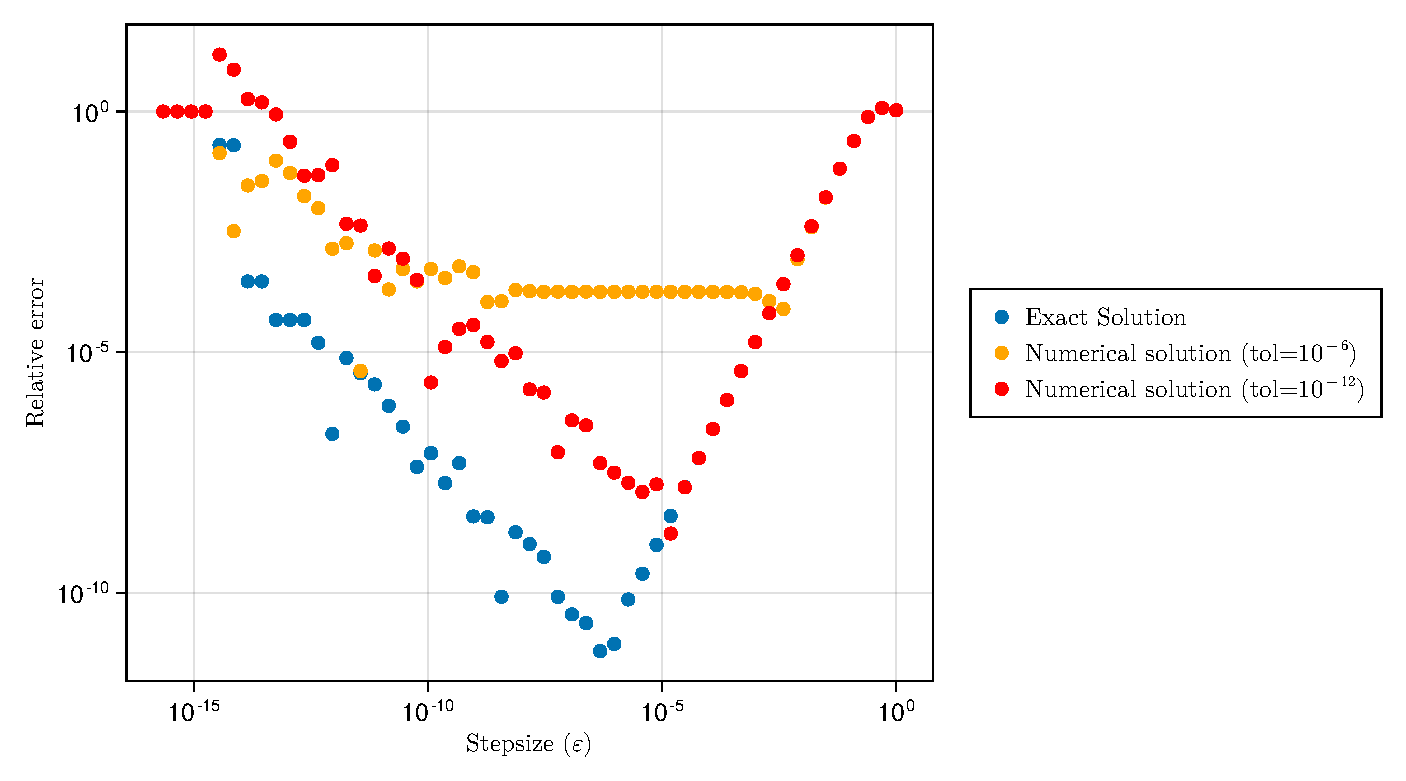
\includegraphics[width=0.85\textwidth]{../code/finite_differences/finite_difference_derivative.pdf}
    \caption{Absolute relative error when computing the gradient of the function $u(t) = \sin (\omega t)/\omega$ with respect to $\omega$ at $t=10.0$ as a function of the stepsize $\varepsilon$. Here $u(t)$ corresponds to the solution of the differential equation $u'' + \omega^2 u = 0$ with initial condition $u(0)=0$ and $u'(0)=1$. The blue dots correspond to the case where this is computed with finite differences. The red and orange lines are for the case where $u(t)$ is numerically computed using the default Tsitouras solver \cite{Tsitouras_2011} from \texttt{OrdinaryDiffEq.jl} using different tolerances. The error when using a numerical solver is larger and it is dependent on the numerical precision of the numerical solver. }
    \label{fig:finite-diff}
\end{figure}

% \subsubsection{Forward-mode AD}

Implementing forward AD using dual numbers is usually carried out using \textit{operator overloading} \cite{Neuenhofen_2018}. 
This means expanding the object associated to a numerical value to include its dual components (derivative) and extending the definition of atomic algebraic functions. 
In Julia, this can be done by relying on multiple dispatch. 
The following example illustrates how to define a dual number and its associated binary addition and multiplication extensions. 
\begin{jllisting}
using Base: @kwdef

@kwdef struct DualNumber{F <: AbstractFloat}
    value::F
    derivative::F
end

# Binary sum
Base.:(+)(a::DualNumber, b::DualNumber) = DualNumber(value = a.value + b.value, derivative = a.derivative + b.derivative)

# Binary product 
Base.:(*)(a::DualNumber, b::DualNumber) = DualNumber(value = a.value * b.value, derivative = a.value*b.derivative + a.derivative*b.value)
\end{jllisting}
We further overload base operations for this new type to extend the definition of standard functions by simply applying the chain rule and storing the derivative in the dual variable following Equation \eqref{eq:dual-number-function}:
\begin{jllisting}
function Base.:(sin)(a::DualNumber)
    value = sin(a.value)
    derivative = a.derivative * cos(a.value)
    return DualNumber(value=value, derivative=derivative)
end
\end{jllisting}
% With all these pieces together, we are able to propagate forward the value of a single-valued derivative through a series of algebraic operations. 
In the Julia ecosystem, \texttt{ForwardDiff.jl} implements forward mode AD with multidimensional dual numbers \cite{RevelsLubinPapamarkou2016}. 
Notice that a major limitation of the dual number approach is that we need a dual variable for each variable we want to differentiate. 
Implementations of forward AD using dual numbers and computational graphs require a number of operations that increases with the number of variables to differentiate, since each computed quantity is accompanied by the corresponding gradient calculations \cite{Griewack-on-AD}. 
This consideration also applies to the other forward methods, including finite differences and complex-step differentiation, which makes forward models inefficient when differentiating with respect to many parameters. 

One of the main challenges in forward AD is how to handle \textit{perturbation confusion} \cite{siskind2005perturbation, manzyuk2019perturbation}.

Notice that both AD based in dual number and complex-step differentiation introduce an abstract unit ($\epsilon$ and $i$, respectively) associated with the imaginary part of the extender value that carries forward the numerical value of the gradient.
% This resemblance between the methods makes them susceptible to the same advantages and disadvantages: easiness of implementation with operator overloading; and inefficient scaling with respect to the number of variables to differentiate. 
Although these methods seem similar, it is important to remark that AD gives the exact gradient, while complex step differentiation relies on numerical approximations that are valid just when the stepsize $\varepsilon$ is small. 
The next example shows how the calculation of the gradient of $\sin (x^2)$ is performed by these two methods:
\begin{equation}
\renewcommand{\arraystretch}{1.5}
\begin{tabular}{@{} l @{\qquad} l @{\qquad} l @{}}
Operation & AD with Dual Numbers  & Complex Step Differentiation \\
$x$ & $x + \epsilon$    & $x + i \varepsilon$ \\
$x^2$ & $x^2 + \epsilon \, (2x)$  & $x^2 - \varepsilon^2 + 2i\varepsilon x$\\
$\sin(x^2)$  & $\sin(x^2) + \epsilon \, \cos(x^2) (2x)$ &
$\sin(x^2 - \varepsilon^2) \cosh (2i\varepsilon) + i \, \cos(x^2 - \varepsilon^2) \sinh (2i\varepsilon)$
\end{tabular}
\label{eq:AD-complex-comparision}
\end{equation}
While the second component of the dual number has the exact derivative of $\sin(x^2)$, it is not until we take $\varepsilon \rightarrow 0$ than we obtain the derivative in the imaginary component for the complex step method
\begin{equation}
    \lim_{\varepsilon \rightarrow 0} \, \frac{1}{\varepsilon} \, \cos(x^2 - \varepsilon^2) \sinh (2i\varepsilon) 
    = 
    \, \cos(x^2) (2x).
\end{equation}
The stepsize dependence of the complex step differentiation method makes it resemble more to finite differences than AD with dual numbers. 
This difference between the methods also makes the complex step method sometimes more efficient than both finite differences and AD \cite{Lantoine_Russell_Dargent_2012}, an effect that can be counterbalanced by the number of extra unnecessary operations that complex arithmetic requires (see last column of \eqref{eq:AD-complex-comparision}) \cite{Martins_Sturdza_Alonso_2003_complex_differentiation}.
It is also important to remark that many modern software already have support for complex number arithmetic, making complex step differentiation very easy to implement.

% \subsubsection{Reverse-mode AD}

The libraries \texttt{ReverseDiff.jl} and \texttt{Zygote.jl} use callbacks to compute gradients. 
When gradients are being computed with less than $\sim 100$ parameters, the former is faster (see documentation).

\cite{Baydin_Pearlmutter_Radul_Siskind_2015}

Notice that the application of reverse AD on a numerical solver (without checkpointing) scales as $\mathcal O (n k)$, with $k$ the number of steps of the numerical solver. 
Furthermore, when reverse AD is applied on the numerical solver, the step-size needs to be adapted to ensure the stability of the backward stesps, further increasing the computational complexity. 

\subsubsection{Further remarks}

A crucial distinction between AD implementations based on computational graphs is between static and dynamical graphs\cite{Baydin_Pearlmutter_Radul_Siskind_2015}. 

\subsection{Solver-based methods}

Sensitivity methods based on numerical solvers tend to be better adapted to the structure and properties of the underlying ODE (stiffness, stability, accuracy) but also more difficult to implement.  
This difficulty arises from the fact that the sensitivity method needs to deal with some numerical and computational considerations, including how to handle matrix/Jacobian-vector products; numerical stability of the forward/backward solver; and memory-time tradeoff. 
These factors are further exacerbated by the number of ODEs and parameters in the model. 
% While explicit methods can be preferable for non-stiff problems, Rosenblock methods can be 
Just a few modern scientific software have the capabilities of handling ODE solvers and computing their sensitivities at the same time. 
The include \texttt{CVODES} within \texttt{SUNDIALS} in C \cite{serban2005cvodes, SUNDIALS-hindmarsh2005sundials}; \texttt{ODESSA} \cite{ODESSA} and \texttt{FATODE} (discrete adjoints) \cite{FATODE2014} both in Fortram; \texttt{SciMLSensitivity.jl} in Julia \cite{rackauckas2020universal}; \texttt{Dolfin-adjoint} based on the \texttt{FEniCS} Project \cite{dolfin2013, dolfin2018}. 

It is important to remark that the underlying machinery of all solvers relies on solvers for linear systems of equations, which can be solved in dense, band (sparse), and Krylow mode. 
% This implies that methods based on numerical solvers are, in principle, more difficult to implement but also more efficient in computing gradients for complex differential equations. 
Another important consideration is that all these methods have subroutines to compute the VJPs involved in the sensitivity and adjoint equations. 
This calculation is carried out by another sensitivity method (finite differences, AD) and this also plays a central role at the moment of analyzing the accuracy and stability of the adjoint method. 

\subsubsection{Sensitivity equation}

\subsubsection{Solving the adjoint}

% Distinctio between discrete and continuous
% Discrete are the exact gradient of the computer program, continuous are not. 
% There is no flexibilty in discrete adjoitns, but there is in continuous
% Human effort required to compute discrete adjoints is large \cite{FATODE2014}

An equally important consideration when working with adjoints is when these are numerically stable. 
Some works have shown that continuous adjoints can lead to unstable sensitivities \cite{Jensen_Nakshatrala_Tortorelli_2014}.
Implicit forward schemes can give rise to explicit backwards schemes, leading to unstable solutions for the gradient. 

\vspace*{10px}
\noindent \textbf{\textit{Solving the backwards mode}}
\vspace*{5px}

The bottleneck of this method is the calculation of the adjoint since in order to solve the adjoint equation we need to know $u(t)$ at any given time. 
Effectively, notice that the adjoint equation involves the terms $f(u, \theta, t)$ and $\frac{\partial h}{\partial u}$ which are both functions of $u(t)$. 
There are different ways of addressing the evaluation of $u(t)$ during the backwards step.
\begin{enumerate}[label=(\roman*)]
    \item \textbf{Dense Store.} During the forward model, we can just store in memory all the intermediate states of the numerical solution. 
    This leads to heavy-memory expensive algorithms. 
    \item \textbf{Re-solve.} Solve again the original ODE together with the adjoint as the solution of the reversed augmented system \cite{chen_neural_2019}
    \begin{equation}
    \frac{d}{dt}
    \begin{bmatrix}
       u \\
       \lambda \\
       \frac{dL}{d\theta}
    \end{bmatrix}
    = 
    \begin{bmatrix}
       -f \\
       - \frac{\partial f}{\partial u}^T \lambda - \frac{\partial h}{\partial u}^T \\
       - \lambda^T \frac{\partial f}{\partial \theta} - \frac{\partial h}{\partial \theta}
    \end{bmatrix}
    % = 
    % - [ 1, \lambda^T, \lambda^T ]
    % \begin{bmatrix}
    %    f & \frac{\partial f}{\partial u} & \frac{\partial f}{\partial \theta} \\
    %    0 & 0 & 0 \\
    %    0 & 0 & 0
    % \end{bmatrix},
    \qquad 
    \begin{bmatrix}
       u \\
       \lambda \\
       \frac{dL}{d\theta}
    \end{bmatrix}(t_1)
    = 
    \begin{bmatrix}
       u(t_1) \\
       \frac{\partial L}{\partial u(t_1)} \\
       \lambda(t_0)^T s(t_0)
    \end{bmatrix}.
    \end{equation}
    However, computing the ODE backwards can be unstable and lead to large numerical errors \cite{kim_stiff_2021, Zhuang_2020}. 
    \item \textbf{Checkpointing. } Also known as windowing, checkpointing is a technique that trade-offs memory and time by saving intermediate states of the solution in the forward pass and recalculating the solution between intermediate states in the backwards mode \cite{Checkpoiting_2023, griewank2008evaluatingderivatives}. 
    This is implemented in \texttt{Checkpointing.jl} \cite{Checkpoiting_2023}.
\end{enumerate} 

One way of solving this system of equations that ensures stability is by using implicit methods. 
However, this requires cubic time in the total number of ordinary differential equations, leading to a total complexity of $\mathcal O((n+p)^3)$ for the adjoint method.
Two alternatives are proposed in \cite{kim_stiff_2021}, the first one called \textit{Quadrature Adjoint} produces a high order interpolation of the solution $u(t)$ as we move forward, then solve for $\lambda$ backwards using an implicit solver and finally integrating $\frac{dL}{d\theta}$ in a forward step.
This reduces the complexity to $\mathcal O (n^3 + p)$, where the cubic cost in the number of ODEs comes from the fact that we still need to solve the original stiff differential equation in the forward step. 
A second but similar approach is to use an implicit-explicit (IMEX) solver, where we use the implicit part for the original equation and the explicit for the adjoint. 
This method also will have complexity $\mathcal O (n^3 + p)$.

\vspace*{10px}
\noindent \textbf{\textit{Solving the quadrature}}
\vspace*{5px}

Another computational consideration is how the integral in Equation \eqref{eq:casa-final-loss-gradient} is numerically evaluated. 
Some methods save computation by noticing that the last step in the continuous adjoint method of evaluating $\frac{dL}{d\theta}$ is an integral instead of an ODE, and then can be evaluated as such without the need to include it in the tolerance calculation inside the numerical solver \cite{that-is-not-an-ode}.
Numerical integration, also known as quadrature integration, consists in approximating integrals by finite sums of the form
Numerical solutions of the integral 
\begin{equation}
    \int_{t_0}^{t_1} 
    F(t) dt
    \approx
    \sum_{i=1}^K \omega_i \, F(\tau_i),
\end{equation}
where the evaluation of the function occurs in certain knots $t_0 \leq \tau_1 < \ldots < \tau_K \leq t_1$, and $\omega_i$ are weights. 
Weights and knots are obtained in order to maximize the order in which polynomials are exactly integrated \cite{stoer2002-numerical}. 

Different quadrature methods are based on different choices of the knots and associated weights.
Between these methods, the Gaussian quadrature is the faster method to evaluate one-dimensional integrals \cite{Norcliffe_gaussquadrature_2023}.

\subsubsection{Computing VJPs}

All the methods analized in this section need to deal with the calculation of VJPs.  
The choice of the specific algorithm to compute VJPs can have significant impact in the overall performance of the sensitivity method. 

In SUNDIALS, the VJPs involved in the sensitivity and adjoint method are handled using finite differences unless specified by the user \cite{SUNDIALS-hindmarsh2005sundials}.
In FATODE, these can be computed with finite differences, AD or provides by the user.

In the Julia ecosystem, different AD packages are available for this task, including \texttt{ForwardDiff.jl}, \texttt{ReverseDiff.jl}, \texttt{Zygote.jl}\cite{Innes_Zygote}, \texttt{Enzyme.jl}\cite{moses_Enzyme}, \texttt{Tracker.jl}.
Each one of these have different advantages depending on scientific problem, computational features, and hardware resources.
This lead to the development of \texttt{AbstractDifferentiation.jl} which allows to combine different methods \cite{Schäfer_Tarek_White_Rackauckas_2021}. 

% \section{Extensions}

% \section{Recommendations}
% % \subsection{General guidelines}

There is no sensitivity method that is universally suitable for all types of DE problems and that performs better under all conditions. 
However, in light of the methods we explore in this work, we can give general guidelines on which methods to use in specific circumstances.
In this section we provide a practical guidance of which methods are the most suitable for different situations. 
A simplified overview of this decision-making process is depicted in Figure \ref{fig:roadmap}. 

\begin{figure}[tb]
    \centering
    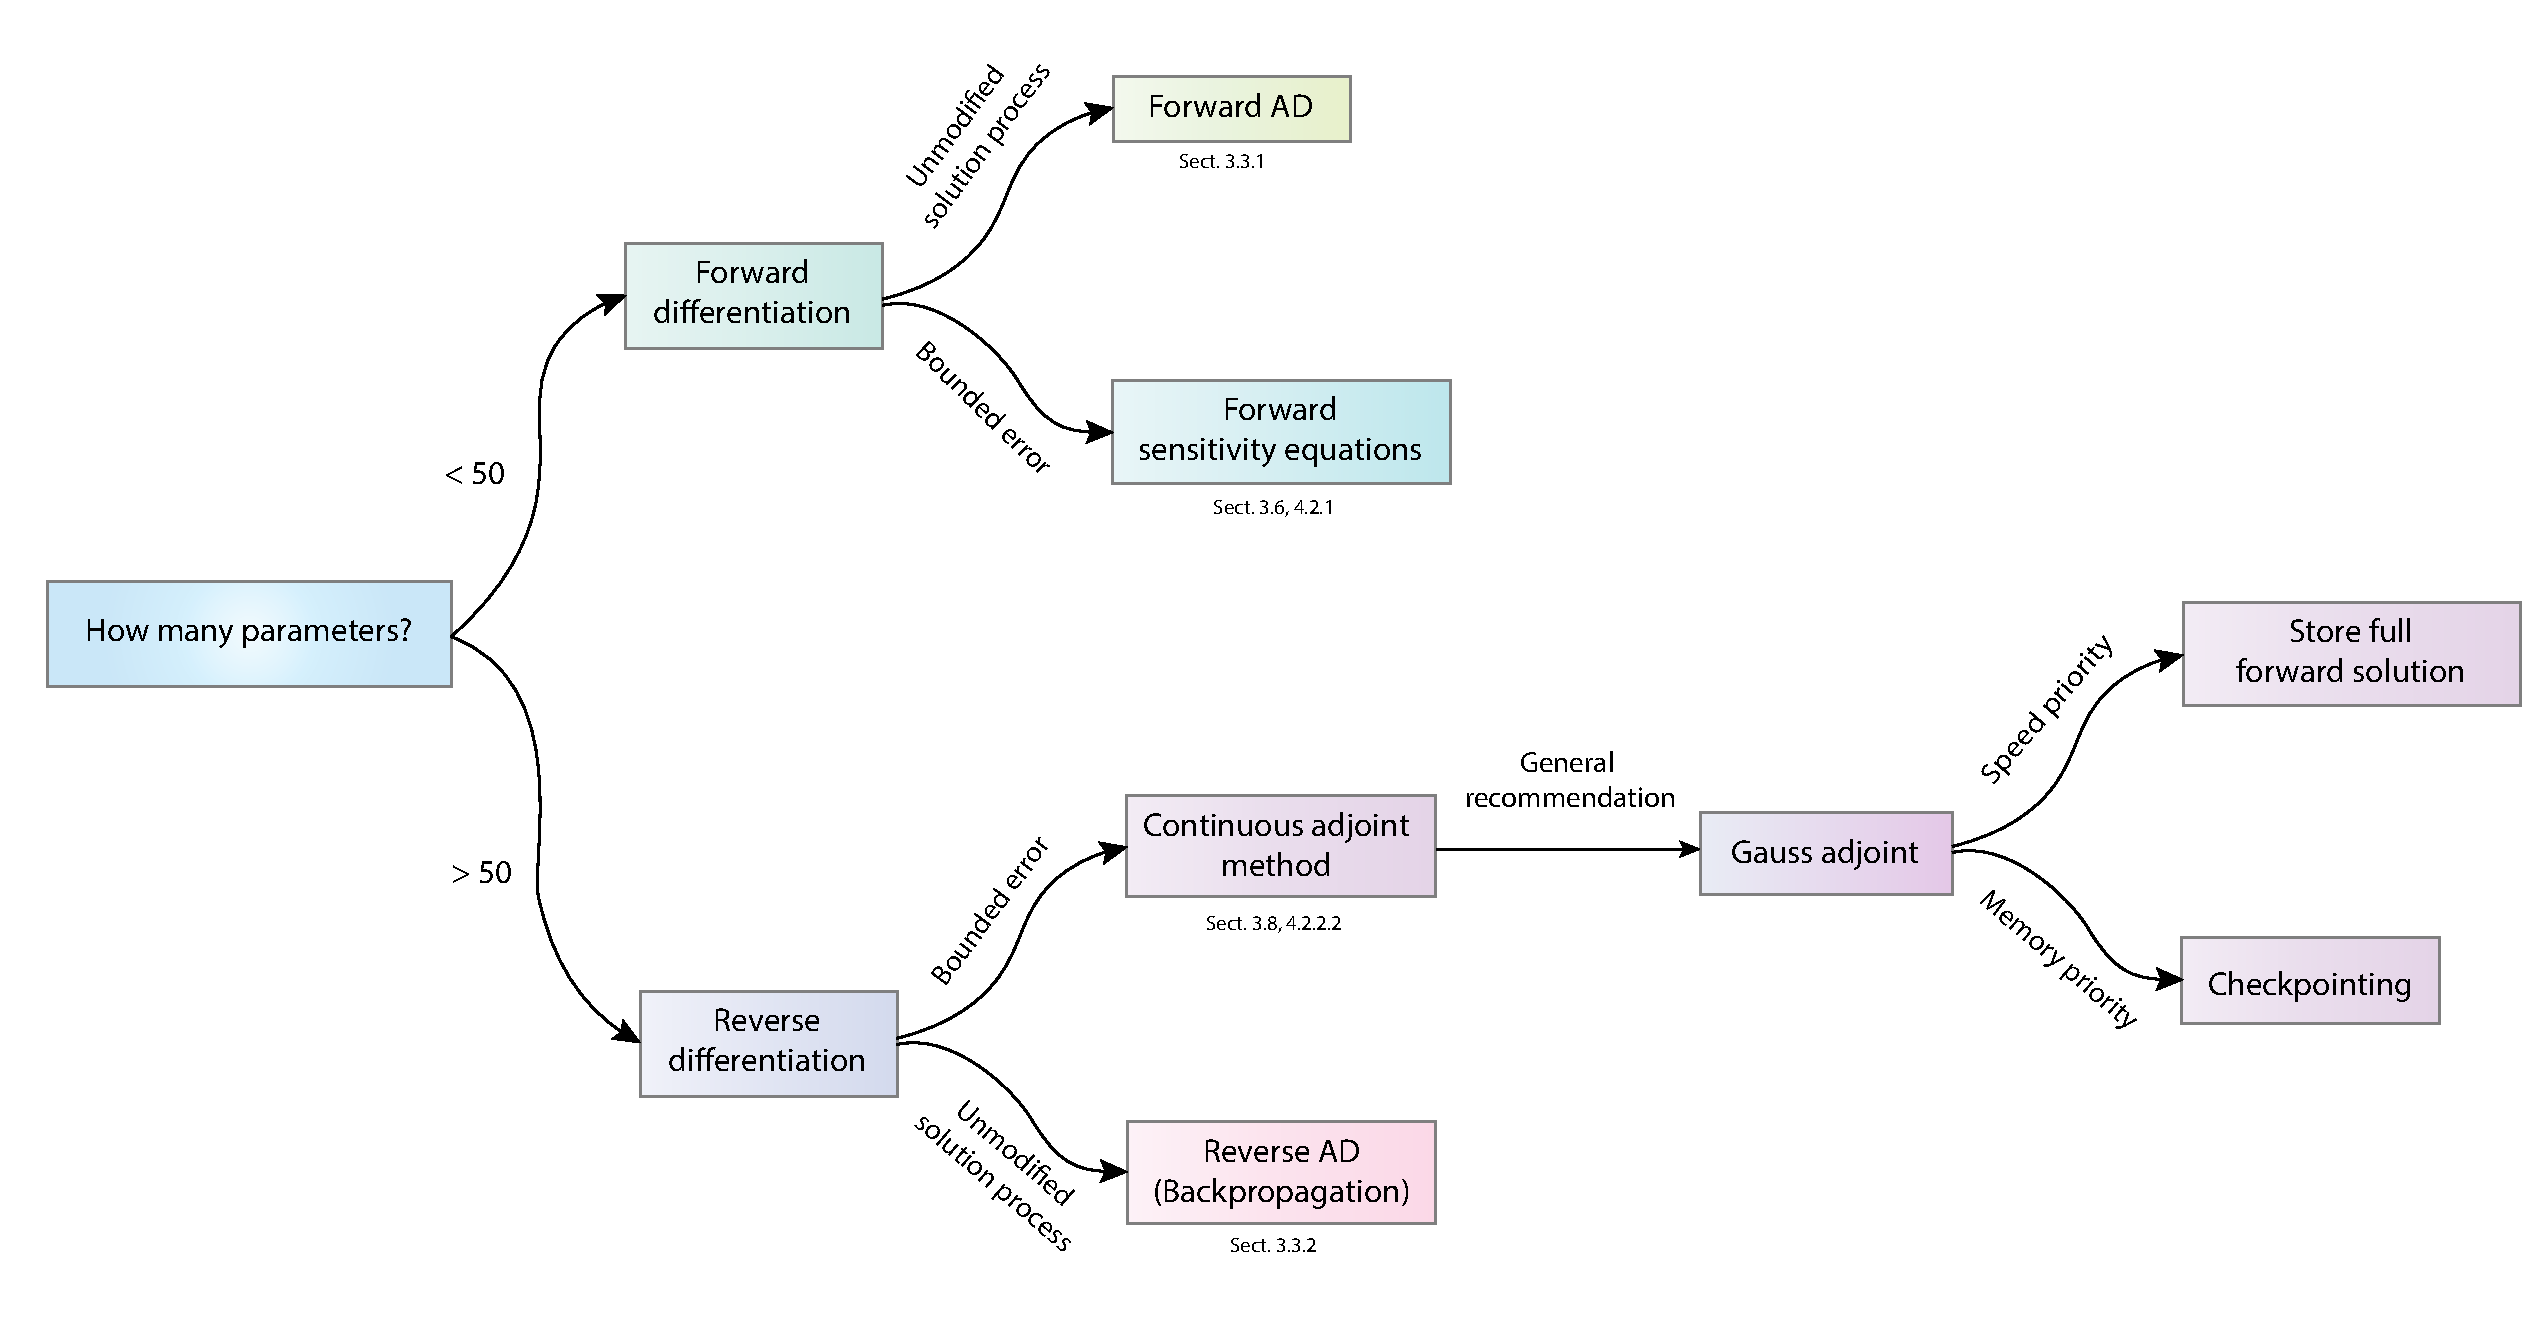
\includegraphics[width=1\textwidth]{tex/figures/roadmap.pdf}
    \caption{Decision-making tree summarizing the choice of sensitivity methods for different problems depending the type of differential equation, number of parameters, and memory-time trade-off.}
    \label{fig:roadmap}
\end{figure}

\subsubsection*{\textit{Working with small systems}}

For sufficiently small systems of less than $50$ parameters and ODEs, that is $n + p < 50$, it has been shown that forward AD and forward sensitivity equations are the most efficient method, outperforming adjoint methods. 
The original benchmark of these methods is included in \cite{ma2021comparison}, though the \texttt{SciMLBenchmarks} system continually updates the benchmarks and has revised the cutoff point as reverse-mode AD engines improved. 
See \url{https://docs.sciml.ai/SciMLBenchmarksOutput/stable/} for continued updates.
Furthermore, as we have shown in Section \ref{section:direct-methods}, AD outperforms other forms of direct differentiation (finite differences, complex-step differentiation). 
Modern scientific software commonly support AD, making forward AD the best choice for small problems. 
% We will make further comments in the choice between discrete and continuous methods later in this section.

\subsubsection*{\textit{Working with large systems}}

For larger systems with either more than 50 parameters plus number of ODEs, reverse techniques are required. 
As explained in section \ref{section:solver-methods}, the continuous adjoint method, particularly the Gauss adjoint, and for very specific cases, the interpolating adjoint and quadrature adjoint, are the most suitable methods to tackle large stiff systems. 
The choice between these three types of adjoints will be problem-specific and will depend on the trade-off between numerical stability, performance and memory usage. 
Adjoint methods supporting checkpointing present more flexibility in this sense, and can allow modulating the method depending on the performance vs memory constraints of each problem. 

Unlike for small systems of ODEs and a reduced number of parameters, differentiating large ODE systems (e.g. stiff discretized PDEs) with respect to a large number of parameters (e.g. in a neural network), is a much more complex problem. 
Current state-of-the-art tools can easily work for a wide array of small systems \cite{rackauckas2020universal}, whereas methods for large systems are still under heavy development and are likely to see many changes and improvements in the future.

% Finally, it is worth mentioning that for complex stiff problems, following different strategies to avoid local minima will be absolutely necessary in order to achieve convergence (.e.g. using multiple shooting \cite{Kiehl:2006tb, Boussange2024} or progressively increasing the time span which is fitted).

\subsubsection*{\textit{Efficiency vs stability}}

When using discrete methods, it is important to be aware that the differentiation machinery is applied after the numerical solver for the differential equation has been specified, meaning that the derivatives are computed with respect to the time discretization instead of the solution \cite{Eberhard_Bischof_1996}.
As discussed in Section \ref{section:software-Forward-AD}, this can mean the method is non-convergent in the case where the iterative solver has adaptive stepsize controllers that depend on the parameter to differentiate.
Although some solutions have been proposed and implemented in Julia to solve this in the case of discrete methods \cite{Eberhard_Bischof_1996}, this is a problem that continuous methods do not have since they apply the differentiation step before the numerical algorithm has been specified. 
Using many of the aforementioned tricks, such as continuous checkpointing and Gaussian quadrature approximations, continuous sensitivity analysis tends to be more memory and computationally efficient. 
However, the errors of discrete adjoint method's derivative error may better represent the actual code being evaluated. 
For this reason, discrete adjoint method have been found in some instances to lead to more stable optimizations. 

In a nutshell, continuous adjoint methods tend to be more efficient while discrete adjoint methods tend to be more stable \cite{rackauckas2020universal}, though the opposite can apply and as such the choice ultimately depends on the nuances of each problem.


\subsubsection*{\textit{Choosing a direct method}}

When computing the gradient of a generic function other than a numerical solver, we further recommend the use of AD (reverse or forward depending the number of parameters) as the direct method of choice, outperforming finite differences, complex step differentiation, and symbolic differentiation. 
This recommendation applies also for the inner VJPs and JVPs calculations performed inside the numerical solver (Section \ref{section:computing-vjp-inside-solver}).
As discussed in Section \ref{section:direct-methods}, finite differences and complex step differentiation do not really provide an advantage over AD in terms of precision and require the tuning of the stepsize $\varepsilon$. 
On the other hand, if symbolic differentiation can be more efficient in nested cases (see ...) or when the spartity pattern of the Jacobian is known, in general this advantage is not drastic in most real cases and can generate difficulties when used inside the numerical solver. 

However, this recommendation is constrained by the availability and interoperability of different AD and sensitivity software. 
For example, when computing higher-order derivatives multiple layers of direct methods became more difficult to implement and may result in complicated computer programs.
In this cases, complex step differentiation may offer an interesting alternative with similar performance than AD for small stepsizes. 
It is important to mention that incorrect implementations of both forward and reverse AD can lead to \textit{perturbation confusion}, an existing problem in some AD software where either repeated applications of AD or differentiation with respect to different dual variables result indistinguishable \cite{siskind2005perturbation, manzyuk2019perturbation}. 


\subsubsection*{\textit{Taking into account model architecture}}
\label{sec:model_arch}

% While it is important to take into account the mathematical aspects of the problem in order to choose the right type of sensitivity method, in practice, c
Code structure and characteristics have a very strong impact in the choice of which packages to use to compute the sensitivities. 
Within the Julia and Python ecosystems, each available AD package implements a specific AD technique which will face certain limitations.
% In the context of Julia and Python, some packages using different AD implementations will be able to deal with certain situations, while others will fail. 
Current limitations include:
\begin{enumerate}[label=(\roman*)]
    \item The use of control flow (i.e. \texttt{if}/\texttt{else} statements; \texttt{for} and \texttt{while} loops) presents issues for dynamic (tape-based) AD methods (see Section \ref{sec:software-reverse-AD}). 
    This is currently not supported by \texttt{ReverseDiff.jl} (with tape compilation) and partially supported by \texttt{JAX} in Python. 
    Non-tape-based AD methods tend to support this, like \texttt{Enzyme.jl} and \texttt{Zygote.jl}.
    \item Mutation of arrays (i.e. in-place operations) is sometimes problematic, since it does not allow to preserve the chain rule during reverse differentation. As such, mutations are not possible for packages like \texttt{Zygote.jl} or \texttt{JAX}. It is however currently supported by \texttt{ReverseDiff.jl} and \texttt{Enzyme.jl}.
    \item Compatibility with GPUs (Graphical Processing Units) is still greatly under development for sensitivity methods. 
    Some AD packages like \texttt{JAX}, \texttt{Enzyme.jl} and \texttt{Zygote.jl} support it, while other packages like \texttt{ReversDiff.jl} do not. 
\end{enumerate}

It is important to bear in mind that direct methods are easier to implement in programming languages where AD already exists and sometimes does not required any special package, like for the Julia programming language.
Nonetheless, users must be aware of the aforementioned convergence issues of AD naively applied to solvers. 
Thus we recommend the use of robust and tested software when available (e.g. the Julia SciML ecosystem or Diffrax in Python) as the solvers must apply corrections to AD implementations in order to guarantee numerically correct derivatives.

% Furthermore, it is important to be aware than when using AD or any other technique we are differentiating the algorithm used to lead to the numerical solution, no the numerical solution itself, which can lead to wrong results \cite{Eberhard_Bischof_1996}.
% When comparing between discrete and continuous methods, more than talking about computational efficiency we are focusing on the mathematical consistency of the method, that is, \textit{is the method estimating the right gradient?}. 
% As we will discuss in the following sections, forward methods are very efficient for problems with a small number of parameters we want to differentiate with respect to, while backwards methods are more efficient for a large number of parameters but they come with a larger memory cost which needs to be overcome using different performance tricks. 
% Neither forward nor reverse mode is more efficient in all cases \cite{Griewank_1989}, as we will discuss in Section \ref{sec:vjp-jvp}.
% When the function to differentiate has a larger input space than output ($q \ll p$), AD in reverse mode is more efficient as it propagates the chain rule by computing VJPs, the reason why reverse-mode AD is more used in modern machine learning.
%  leading to performance overhead that makes forward AD more efficient when $p \lesssim q$
% The former are easier to implement since they are agnostic with respect to the mathematical and numerical properties of the system of ODEs; however, they tend to be either inaccurate, memory-expensive, or at times unfeasible for large models. 
% which makes forward models prone to the curse of dimensionality with respect to the number of parameters considered
% For complex and large systems, direct methods for computing the gradient on top of the numerical solver can be memory expensive due to the large number of function evaluations required by the solver and the later store of the intermediate states. 


% See recommendations at \cite{Shen_diff_modelling}.

% \section{Conclusions}
% 
We also encourage the interested reader to direct their attention to other comprehensive works on automatic differentiation \cite{Baydin_Pearlmutter_Radul_Siskind_2015}; adjoint methods, ...

% \section{Do we need full gradients?}

% \section{Notation}
% \setlength{\tabcolsep}{10pt} % Default value: 6pt
\renewcommand{\arraystretch}{1.2}
\begin{table}[H]
    \center
    \begin{tabular}{| p{3cm} | p{8cm} |}
    \hline
    Variable            & Meaning \\ [0.5ex] 
    \hline  
    $u$					& Solution of the differential equation \\
    $\theta$            & Parameters of the model \\
    $L$ 				& Loss function \\
    $s$                 & Sensitivity of the solution given by $\frac{\partial u}{\partial \theta}$ \\
    $n$                 & Number of ODEs \\
    $p$                 & Number of parameters \\
    \hline
\end{tabular}	
\end{table}


\newpage
\appendix
\section*{Appendices}
\addcontentsline{toc}{section}{Appendices}
\renewcommand{\thesubsection}{\Alph{subsection}}

\subsection{Lagrangian derivation of adjoints}
\label{appendix:lagrangian}

%by the means of the \emph{Lagrange multiplier method}\cite{Vadlamani.2020}.
% The introduction of the adjoint variable allows to reduce the computational complexity of sensitivity methods, as we will explore in this section and later in Section \ref{section:computing-adjoints}.

The adjoint equation can be derived directly from the 
Following the analysis in \cite{Giles_Pierce_2000}, we decided to present both approaches here, although we prefer with the duality viewpoint introduced in the main text since we believe is more commonly used and easy to understand for newcomers. 

In this section we are going to derive the adjoint equation for both discrete and continuous methods using the Lagrangian formulation of the adjoint. 
It is important to mention that this is different than using the Lagrange multipliers approach, a common confusion in the literature\cite{Givoli_2021}.
Conceptually, the method is the same in both discrete and continuous case, with the difference that we manipulate linear algebra objects for the former and continuous operators for the later. 

\subsubsection{Discrete adjoint}

\subsubsection{Continuous adjoint}

For the continuous adjoint method, we proceed the same way by writing a new loss function $I(\theta)$, sometimes known as the \textit{Lagrangian}, identical to $L(\theta)$ as 
\begin{equation}
    I(\theta) = L(\theta) - \inttime \lambda(t)^T \left( \frac{du}{dt} - f(u, \theta, t) \right) dt
\end{equation}
where $\lambda(t) \in \mathbb R^n$ is the Lagrange multiplier of the continuous constraint defined by the differential equation. Now, 
\begin{equation}
    \frac{dL}{d\theta} = \frac{dI}{d\theta} = 
    \inttime \left( \frac{\partial h}{\partial \theta} + \frac{\partial h}{\partial u} \frac{\partial u}{\partial \theta} \right) dt
    - 
    \inttime \lambda(t)^T \left( \frac{d}{dt} \frac{du}{d\theta} - \frac{\partial f}{\partial u} \frac{du}{d\theta} - \frac{\partial f}{\partial \theta} \right) dt.
\end{equation}
Notice that the term involved in the second integral is the same we found when deriving the sensitivity equations. 
We can derive an easier expression for the last term using integration by parts. 
Using our usual definition of the sensitivity $s = \frac{du}{d\theta}$, and performing integration by parts in the term $\lambda^T \frac{d}{dt} \frac{du}{d\theta}$ we derive 
\begin{multline}
    \frac{dL}{d\theta}
    = 
    \inttime \left( \frac{\partial h}{\partial \theta} + \lambda^T \frac{\partial f}{\partial \theta} \right) dt 
    - 
    \inttime \left( - \frac{d\lambda^T}{dt} - \lambda^T \frac{\partial f}{\partial u} - \frac{\partial h}{\partial u} \right) \, s(t) \, dt \\
    -
    \bigg ( \lambda(t_1)^T s(t_1) - \lambda(t_0)^T s(t_0) \bigg ).
    \label{eq:continous-adjoint-loss}
\end{multline}
Now, we can force some of the terms in the last equation to be zero by solving the following adjoint differential equation for $\lambda(t)^T$ in backwards mode
\begin{equation}
    \frac{d\lambda}{d\theta} = - \left(\frac{\partial f}{\partial u}\right)^T \lambda - \left( \frac{\partial h}{\partial u} \right)^T,
    \label{eq:continuous-adjoint}
\end{equation}
with final condition $\lambda(t_1) = 0$. 

It is easy to see that this derivation is equivalent to solving the Karush-Kuhn-Tucker (KKT) conditions. 

\subsection{Supplementaty code}
This is a list of the code provided along with the current manuscript.
All the following scripts can be found in the GitHub repository \href{https://github.com/ODINN-SciML/DiffEqSensitivity-Review}{\texttt{DiffEqSensitivity-Review}}. 
 
\begin{itemize}
    \item[$\clubsuit_\text{\ref{code:figure-comparison}}$] \textbf{Comparison of direct methods.} The script \href{https://github.com/ODINN-SciML/DiffEqSensitivity-Review/blob/main/code/DirectMethods/Comparison/direct-comparision.jl}{\texttt{direct-comparision.jl}} reproduces Figure \ref{fig:direct-methods}.
    \item[$\clubsuit_\text{\ref{code:dual-number}}$] \textbf{Dual numbers definition.} The script \href{https://github.com/ODINN-SciML/DiffEqSensitivity-Review/blob/main/code/DirectMethods/DualNumbers/dualnumber_definition.jl}{\texttt{dualnumber\_definition.jl}} includes a very simple example of how to define a dual number using \texttt{struct} in Julia and how to extend simple unary and binary operations to implement the chain rule usign multiple distpatch. 
    \item[$\clubsuit_\text{\ref{code:AD-wrong}}$] \textbf{When AD is algorithmically correct but numerically wrong.} The script \href{https://github.com/ODINN-SciML/DiffEqSensitivity-Review/blob/main/code/SensitivityForwardAD/example-AD-tolerances.jl}{\texttt{example-AD-tolerances.jl}} includes the example shown in Section \ref{section:software-Forward-AD} and further elaborated in Section \ref{section:AD-incorrect} where forward AD gives the wrong answer when tolerances in the gradient are not computed taking into account both numerical errors in the numerical solution and the sensitivity matrix. Further examples of this phenomena can be found in the  and the Julia \href{https://github.com/ODINN-SciML/DiffEqSensitivity-Review/blob/main/code/SensitivityForwardAD/testgradient_julia.jl}{\texttt{testgradient\_julia.jl}}.
    \item[$\clubsuit_\text{\ref{code:AD-wrong-JAX}}$] \textbf{When AD is algorithmically correct but numerically wrong (JAX)}. Python script \href{https://github.com/ODINN-SciML/DiffEqSensitivity-Review/blob/main/code/SensitivityForwardAD/testgradient_python.py}{\texttt{testgradient\_python.py}}
    \item[$\clubsuit_\text{\ref{code:complex-step}}$] \textbf{Complex step in numerical solver.} The script \href{https://github.com/ODINN-SciML/DiffEqSensitivity-Review/blob/main/code/DirectMethods/ComplexStep/complex_solver.jl}{\texttt{complex\_solver.jl}} shows how to define the dynamics of the ODE to support complex variables and then compute the complex step derivative. 
    \item[$\clubsuit_\text{\ref{code:sensitivity-equation}}$] \textbf{Solving the forward sensitivity equation. } The scrip \href{https://github.com/ODINN-SciML/DiffEqSensitivity-Review/blob/main/code/SolverMethods/Harmonic/forward_sensitivity_equations.jl}{\texttt{forward_sensitivity_equations.jl}} includes a manual implementation of the  forward sensitivity equations. This also includes how to compute the same sensitivity using \texttt{ForwardSensitivity} in Julia. 
    \item[$\clubsuit_\text{\ref{code:discrete-adjoint}}$] The script \href{https://github.com/ODINN-SciML/DiffEqSensitivity-Review/blob/main/code/SolverMethods/Harmonic/adjoint_discrete.jl}{\texttt{adjoint_discrete.jl}} includes a manual implementation of the discrete adjoint method for the simple harmonic oscillator. 
\end{itemize}

% \section{Glossary} 

\newpage
\printbibliography[heading=bibintoc, title={References}]

\end{document}